% Capitolul 3: Distribuții α-stabile
% Statistica piețelor financiare -- Program de licență, Academia de Studii Economice din București
% GENERAT de latex/build_chapter3.py -- modificați generatorul, nu acest fișier.

\newcommand{\coursename}{Statistica piețelor financiare}
\def\sfmlang{ro}
% Preambul comun SFM -- Statistica piețelor financiare / Statistics of Financial Markets (Beamer, 16:9)
% Același design ca MFM. Înainte de % Preambul comun SFM -- Statistica piețelor financiare / Statistics of Financial Markets (Beamer, 16:9)
% Același design ca MFM. Înainte de % Preambul comun SFM -- Statistica piețelor financiare / Statistics of Financial Markets (Beamer, 16:9)
% Același design ca MFM. Înainte de \input{../../latex/preamble} se definește
%   \newcommand{\coursename}{Statistics of Financial Markets}      (EN)
%   \newcommand{\coursename}{Statistica piețelor financiare}       (RO)  și  \def\sfmlang{ro}
% Fișierele .tex se află în EN/Courses, EN/Seminars, RO/Cursuri, RO/Seminarii (două niveluri sub rădăcină).
% Deck-urile sînt generate de latex/build_chapterN.py / build_seminarN.py (vezi latex/sfm_build.py).

\documentclass[9pt, aspectratio=169, t]{beamer}
\providecommand{\coursename}{Statistics of Financial Markets}

% Ensure content fits on slides
\setbeamersize{text margin left=8mm, text margin right=8mm}

%=============================================================================
% THEME AND STYLE CONFIGURATION
%=============================================================================
\usetheme{default}
% Using default theme for clean header/footer control

% Color Palette (matching Redispatch PDF)
\definecolor{MainBlue}{RGB}{26, 58, 110}
\definecolor{AccentBlue}{RGB}{26, 58, 110}
\definecolor{IDAred}{RGB}{205, 0, 0}
\definecolor{DarkGray}{RGB}{51, 51, 51}
\definecolor{MediumGray}{RGB}{128, 128, 128}
\definecolor{LightGray}{RGB}{248, 248, 248}
\definecolor{VeryLightGray}{RGB}{235, 235, 235}
\definecolor{KeynoteGray}{RGB}{218, 218, 218}
\definecolor{SectionGray}{RGB}{120, 120, 120}
\definecolor{FooterGray}{RGB}{100, 100, 100}
\definecolor{Crimson}{RGB}{220, 53, 69}
\definecolor{Forest}{RGB}{46, 125, 50}
\definecolor{Amber}{RGB}{181, 133, 63}
\definecolor{Orange}{RGB}{230, 126, 34}
\definecolor{Purple}{RGB}{142, 68, 173}

% Gradient background (exact Keynote 315° gradient: white to RGB 218,218,218)
\setbeamertemplate{background}{%
    \begin{tikzpicture}[remember picture, overlay]
        \shade[shading=axis, shading angle=315,
        top color=white, bottom color=KeynoteGray]
        (current page.south west) rectangle (current page.north east);
    \end{tikzpicture}%
}
% Fallback solid color for compatibility
\setbeamercolor{background canvas}{bg=}

\setbeamercolor{palette primary}{bg=MainBlue, fg=white}
\setbeamercolor{palette secondary}{bg=MainBlue!85, fg=white}
\setbeamercolor{palette tertiary}{bg=MainBlue!70, fg=white}
\setbeamercolor{structure}{fg=MainBlue}
\setbeamercolor{title}{fg=IDAred}
\setbeamercolor{frametitle}{fg=IDAred, bg=}
\setbeamercolor{block title}{bg=MainBlue, fg=white}
\setbeamercolor{block body}{bg=VeryLightGray, fg=DarkGray}
\setbeamercolor{block title alerted}{bg=Crimson, fg=white}
\setbeamercolor{block body alerted}{bg=Crimson!8, fg=DarkGray}
\setbeamercolor{block title example}{bg=Forest, fg=white}
\setbeamercolor{block body example}{bg=Forest!8, fg=DarkGray}
\setbeamercolor{item}{fg=MainBlue}

% Footer colors (override Madrid theme blue)
\setbeamercolor{author in head/foot}{fg=FooterGray, bg=}
\setbeamercolor{title in head/foot}{fg=FooterGray, bg=}
\setbeamercolor{date in head/foot}{fg=FooterGray, bg=}
\setbeamercolor{section in head/foot}{fg=FooterGray, bg=}
\setbeamercolor{subsection in head/foot}{fg=FooterGray, bg=}

% Bullet styles (apply everywhere including blocks)
\setbeamertemplate{itemize item}{\color{MainBlue}$\boxdot$}
\setbeamertemplate{itemize subitem}{\color{MainBlue}$\blacktriangleright$}
\setbeamertemplate{itemize subsubitem}{\color{MainBlue}\tiny$\bullet$}
\setbeamertemplate{itemize/enumerate body begin}{\normalsize}
\setbeamertemplate{itemize/enumerate subbody begin}{\normalsize}

% Item spacing - compact style
\setlength{\leftmargini}{10pt}       % Level 1: minimal indent
\setlength{\leftmarginii}{10pt}      % Level 2: minimal additional indent
% Compact list spacing (zero extra space before/after lists in blocks)
\makeatletter
\def\@listi{\leftmargin\leftmargini \topsep 0pt \parsep 0pt \itemsep 0pt}
\def\@listii{\leftmargin\leftmarginii \topsep 0pt \parsep 0pt \itemsep 0pt}
\makeatother

\setbeamertemplate{navigation symbols}{}

%=============================================================================
% CUSTOM HEADLINE
%=============================================================================
\setbeamertemplate{headline}{%
    \vskip10pt%
    \hbox to \paperwidth{%
        \hskip0.5cm%
        {\small\color{FooterGray}\renewcommand{\hyperlink}[2]{##2}\insertsectionhead}%
        \hfill%
        \textcolor{FooterGray}{\small\insertframenumber}%
        \hskip0.5cm%
    }%
    \vskip4pt%
    {\color{FooterGray}\hrule height 0.4pt}%
}

%=============================================================================
% CUSTOM FOOTER
%=============================================================================
\usepackage{fontawesome5}

\setbeamertemplate{footline}{%
    {\color{FooterGray}\hrule height 0.4pt}%
    \vskip4pt%
    \hbox to \paperwidth{%
        \hskip0.5cm%
        \textcolor{FooterGray}{\small\coursename}%
        \hfill%
        \raisebox{-0.1em}{%
            \begin{tikzpicture}[x=0.08em, y=0.08em, line width=0.4pt]
                \draw[FooterGray] (0,3) -- (1,4) -- (2,3.5) -- (3,5) -- (4,4) -- (5,6) -- (6,5.5) -- (7,4) -- (8,5) -- (9,7) -- (10,6) -- (11,5) -- (12,6.5) -- (13,8) -- (14,7) -- (15,6) -- (16,7.5) -- (17,9) -- (18,8) -- (19,7) -- (20,8.5) -- (21,10) -- (22,9) -- (23,8) -- (24,9.5);
            \end{tikzpicture}%
        }%
        \hskip0.5cm%
    }%
    \vskip6pt%
}

%=============================================================================
% PACKAGES
%=============================================================================
\usepackage[utf8]{inputenc}
\DeclareUnicodeCharacter{03B1}{\ensuremath{\alpha}}
\usepackage[T1]{fontenc}
\usepackage{amsmath, amssymb, amsthm}
\usepackage{mathtools}
\usepackage{bm}
\usepackage{tikz}
\usetikzlibrary{arrows.meta, positioning, shapes, calc, decorations.pathreplacing, shadings}
\usepackage{booktabs}
\usepackage{multirow}
\usepackage{array}
\usepackage{graphicx}
\usepackage{hyperref}
\usepackage{colortbl}
\usepackage{listings}
\lstset{language=Python, basicstyle=\ttfamily\scriptsize, keywordstyle=\color{MainBlue}\bfseries,
  commentstyle=\color{Forest}, stringstyle=\color{Crimson}, breaklines=true,
  frame=none, backgroundcolor=\color{VeryLightGray}, xleftmargin=2mm}
\hypersetup{colorlinks=true, linkcolor=MainBlue, urlcolor=MainBlue}
\graphicspath{{../../logos/}{../../charts/}{../../photos/}}
\usepackage{xcolor}
\hfuzz=2pt  % Suppress tiny overfull warnings (<2pt)
\vfuzz=2pt  % Suppress tiny vertical overfull warnings (<2pt)

%=============================================================================
% QUANTLET COMMANDS
%   \quantlet{<displayed name>}{<url>}       (generic, compatible with the older SFM decks)
%   \sfmquantlet{Ch_05}{SFM_ch5_garch}       -> https://github.com/danpele/SFM/tree/main/Quantlets/Ch_05/SFM_ch5_garch
%   \qlurl{<folder>} is defined per chapter by the generator (Quantlets/Ch_NN/<folder>)
%=============================================================================
\newcommand{\sfmrepo}{https://github.com/danpele/SFM}
\newcommand{\sfmqlbase}{https://github.com/danpele/SFM/tree/main/Quantlets}
\newcommand{\quantlet}[2]{%
    \hfill\href{#2}{%
        \raisebox{-0.15em}{
\includegraphics[height=0.7em]{ql_logo.png}}%
        \textcolor{MainBlue}{\tiny\ #1}%
    }%
}
\newcommand{\sfmquantlet}[2]{\quantlet{\detokenize{#2}}{\sfmqlbase/#1/#2}}

%=============================================================================
% NOTEBOOKS (Google Colab)
%   \colaburl{notebooks/EN/chapter5_seminar_notebook.ipynb} -> the Colab link of a file in the SFM repo
%   \nb: the chapter notebook (each seminar deck redefines it with \renewcommand)
%=============================================================================
\newcommand{\colaburl}[1]{https://colab.research.google.com/github/danpele/SFM/blob/main/#1}
\newcommand{\nb}{https://colab.research.google.com/github/danpele/SFM/tree/main/notebooks/EN}
\newcommand{\nbname}{notebooks/EN}

%=============================================================================
% SLIDE HELPERS (used by the generators; the same as in MFM)
%=============================================================================
% local font size for list bodies (the preamble forces \normalsize)
\newcommand{\itemsize}[1]{\setbeamertemplate{itemize/enumerate body begin}{#1}\setbeamertemplate{itemize/enumerate subbody begin}{#1}}
\newcommand{\intitle}[1]{{\hypersetup{urlcolor=white}#1}}   % white links inside coloured title bars
\newcommand{\imgcap}[1]{{\scriptsize #1}\\[0.5mm]}          % caption under a photo
\newcommand{\imgcredit}[2]{{\tiny\color{FooterGray}\href{#1}{#2}}}   % image credit: source URL, author/licence
\newcommand{\aiprompt}[1]{{\ttfamily\color{MainBlue}#1}}     % a prompt to an AI assistant

%=============================================================================
% SEMINARS: student version by default; the instructor wrapper *_solutions.tex sets \solutionstrue
%=============================================================================
\makeatletter\@ifundefined{ifsolutions}{\expandafter\newif\csname ifsolutions\endcsname}{}\makeatother
\newcommand{\solonly}[1]{\ifsolutions #1\fi}
\newcommand{\propsub}{\ifsolutions\else\framesubtitle{\ifdefined\sfmlang Rezolvarea se discută la seminar\else Solution discussed in class\fi}\fi}

%=============================================================================
% APPENDIX AND CHAPTER LINKS (latex/appendix_links.py writes the calls; it also re-declares these
% macros before \begin{document}, so the decks compile with or without this preamble block)
%=============================================================================
\providecommand{\sfmapplink}[3]{\hypertarget{#2}{}\hyperlink{#1}{\beamergotobutton{#3}}}
\providecommand{\sfmappback}[2]{\begin{tikzpicture}[remember picture,overlay]\node[anchor=south east] at ([xshift=-3mm,yshift=7mm]current page.south east){\hyperlink{#1}{\beamerreturnbutton{#2}}};\end{tikzpicture}}
\providecommand{\sfmchlink}[2]{\href{#1}{#2}}
\providecommand{\sfmchlinkt}[2]{\href{#1}{\usebeamercolor[fg]{frametitle}#2}}

%=============================================================================
% QUANTINAR COMMAND: link către un curs Quantinar (subiecte avansate)
%=============================================================================
\newcommand{\quantinar}[2]{%
    \href{#2}{%
        \raisebox{-0.15em}{
\includegraphics[height=0.8em]{qr_logo.png}}%
        \textcolor{MainBlue}{\scriptsize\ #1}%
    }%
}

%=============================================================================
% CUSTOM TITLE PAGE
%=============================================================================
\defbeamertemplate*{title page}{hybrid}[1][]
{
    \vspace{0.2cm}
    % Logos row - top header (with clickable links)
    \begin{center}
        \href{https://www.ase.ro}{
\includegraphics[height=1.0cm]{ase_logo.png}}\hspace{0.3cm}%
        \href{https://theida.net}{
\includegraphics[height=1.0cm]{ida_logo.png}}\hspace{0.3cm}%
        \href{https://blockchain-research-center.com}{
\includegraphics[height=1.0cm]{brc_logo.png}}\hspace{0.3cm}%
        \href{https://www.ai4efin.ase.ro}{
\includegraphics[height=1.0cm]{ai4efin_logo.png}}\hspace{0.3cm}%
        \href{https://ipe.ro/new}{
\includegraphics[height=1.0cm]{acad_logo.png}}\hspace{0.3cm}%
        \href{https://www.digital-finance-msca.com}{
\includegraphics[height=1.0cm]{msca_logo.png}}%
    \end{center}

    \vspace{0.6cm}

    % Main title with Q logos on sides (with clickable links)
    \begin{center}
        \begin{minipage}{0.1\textwidth}
            \centering
            \href{https://quantlet.com}{
\includegraphics[height=1.1cm]{ql_logo.png}}
        \end{minipage}%
        \begin{minipage}{0.78\textwidth}
            \centering
            {\LARGE\bfseries\usebeamercolor[fg]{title}\inserttitle}

            \vspace{0.3cm}

            {\usebeamerfont{subtitle}\usebeamercolor[fg]{title}\insertsubtitle}
        \end{minipage}%
        \begin{minipage}{0.1\textwidth}
            \centering
            \href{https://quantinar.com}{
\includegraphics[height=1.1cm]{qr_logo.png}}
        \end{minipage}
    \end{center}

    \vspace{0.6cm}

    % Authors (left aligned)
    \hspace{0.5cm}{\usebeamerfont{author}\insertauthor}

    \vspace{0.3cm}

    % Institute/Affiliations (left aligned)
    \hspace{0.5cm}\begin{minipage}[t]{0.9\textwidth}
        \raggedright\small\insertinstitute
    \end{minipage}
}

%=============================================================================
% THEOREM ENVIRONMENTS
%=============================================================================
\theoremstyle{definition}
\setbeamertemplate{theorems}[numbered]
\ifdefined\sfmlang
\newtheorem{defn}{Definiție}
\newtheorem{thm}{Teoremă}
\newtheorem{prop}{Propoziție}
\newtheorem{rmk}{Observație}
\else
\newtheorem{defn}{Definition}
\newtheorem{thm}{Theorem}
\newtheorem{prop}{Proposition}
\newtheorem{rmk}{Remark}
\fi

%=============================================================================
% CENTRED MINIPAGE (no extra vertical space)
%=============================================================================
\newenvironment{cminipage}[1]{%
    \par\noindent\hfill\begin{minipage}{#1}\ignorespaces
}{%
    \end{minipage}\hfill\null\par
}

%=============================================================================
% CUSTOM COMMANDS
%=============================================================================
\newcommand{\E}{\mathbb{E}}
\newcommand{\Var}{\text{Var}}
\newcommand{\Cov}{\text{Cov}}
\newcommand{\Corr}{\text{Corr}}
\newcommand{\R}{\mathbb{R}}
\newcommand{\N}{\mathbb{N}}
\newcommand{\Z}{\mathbb{Z}}
\newcommand{\B}{\mathbf{B}}
\newcommand{\imark}{\textcolor{MainBlue}{\textbullet}}
\newcommand{\RMSE}{\text{RMSE}}
\newcommand{\MAE}{\text{MAE}}
\newcommand{\MAPE}{\text{MAPE}}

 se definește
%   \newcommand{\coursename}{Statistics of Financial Markets}      (EN)
%   \newcommand{\coursename}{Statistica piețelor financiare}       (RO)  și  \def\sfmlang{ro}
% Fișierele .tex se află în EN/Courses, EN/Seminars, RO/Cursuri, RO/Seminarii (două niveluri sub rădăcină).
% Deck-urile sînt generate de latex/build_chapterN.py / build_seminarN.py (vezi latex/sfm_build.py).

\documentclass[9pt, aspectratio=169, t]{beamer}
\providecommand{\coursename}{Statistics of Financial Markets}

% Ensure content fits on slides
\setbeamersize{text margin left=8mm, text margin right=8mm}

%=============================================================================
% THEME AND STYLE CONFIGURATION
%=============================================================================
\usetheme{default}
% Using default theme for clean header/footer control

% Color Palette (matching Redispatch PDF)
\definecolor{MainBlue}{RGB}{26, 58, 110}
\definecolor{AccentBlue}{RGB}{26, 58, 110}
\definecolor{IDAred}{RGB}{205, 0, 0}
\definecolor{DarkGray}{RGB}{51, 51, 51}
\definecolor{MediumGray}{RGB}{128, 128, 128}
\definecolor{LightGray}{RGB}{248, 248, 248}
\definecolor{VeryLightGray}{RGB}{235, 235, 235}
\definecolor{KeynoteGray}{RGB}{218, 218, 218}
\definecolor{SectionGray}{RGB}{120, 120, 120}
\definecolor{FooterGray}{RGB}{100, 100, 100}
\definecolor{Crimson}{RGB}{220, 53, 69}
\definecolor{Forest}{RGB}{46, 125, 50}
\definecolor{Amber}{RGB}{181, 133, 63}
\definecolor{Orange}{RGB}{230, 126, 34}
\definecolor{Purple}{RGB}{142, 68, 173}

% Gradient background (exact Keynote 315° gradient: white to RGB 218,218,218)
\setbeamertemplate{background}{%
    \begin{tikzpicture}[remember picture, overlay]
        \shade[shading=axis, shading angle=315,
        top color=white, bottom color=KeynoteGray]
        (current page.south west) rectangle (current page.north east);
    \end{tikzpicture}%
}
% Fallback solid color for compatibility
\setbeamercolor{background canvas}{bg=}

\setbeamercolor{palette primary}{bg=MainBlue, fg=white}
\setbeamercolor{palette secondary}{bg=MainBlue!85, fg=white}
\setbeamercolor{palette tertiary}{bg=MainBlue!70, fg=white}
\setbeamercolor{structure}{fg=MainBlue}
\setbeamercolor{title}{fg=IDAred}
\setbeamercolor{frametitle}{fg=IDAred, bg=}
\setbeamercolor{block title}{bg=MainBlue, fg=white}
\setbeamercolor{block body}{bg=VeryLightGray, fg=DarkGray}
\setbeamercolor{block title alerted}{bg=Crimson, fg=white}
\setbeamercolor{block body alerted}{bg=Crimson!8, fg=DarkGray}
\setbeamercolor{block title example}{bg=Forest, fg=white}
\setbeamercolor{block body example}{bg=Forest!8, fg=DarkGray}
\setbeamercolor{item}{fg=MainBlue}

% Footer colors (override Madrid theme blue)
\setbeamercolor{author in head/foot}{fg=FooterGray, bg=}
\setbeamercolor{title in head/foot}{fg=FooterGray, bg=}
\setbeamercolor{date in head/foot}{fg=FooterGray, bg=}
\setbeamercolor{section in head/foot}{fg=FooterGray, bg=}
\setbeamercolor{subsection in head/foot}{fg=FooterGray, bg=}

% Bullet styles (apply everywhere including blocks)
\setbeamertemplate{itemize item}{\color{MainBlue}$\boxdot$}
\setbeamertemplate{itemize subitem}{\color{MainBlue}$\blacktriangleright$}
\setbeamertemplate{itemize subsubitem}{\color{MainBlue}\tiny$\bullet$}
\setbeamertemplate{itemize/enumerate body begin}{\normalsize}
\setbeamertemplate{itemize/enumerate subbody begin}{\normalsize}

% Item spacing - compact style
\setlength{\leftmargini}{10pt}       % Level 1: minimal indent
\setlength{\leftmarginii}{10pt}      % Level 2: minimal additional indent
% Compact list spacing (zero extra space before/after lists in blocks)
\makeatletter
\def\@listi{\leftmargin\leftmargini \topsep 0pt \parsep 0pt \itemsep 0pt}
\def\@listii{\leftmargin\leftmarginii \topsep 0pt \parsep 0pt \itemsep 0pt}
\makeatother

\setbeamertemplate{navigation symbols}{}

%=============================================================================
% CUSTOM HEADLINE
%=============================================================================
\setbeamertemplate{headline}{%
    \vskip10pt%
    \hbox to \paperwidth{%
        \hskip0.5cm%
        {\small\color{FooterGray}\renewcommand{\hyperlink}[2]{##2}\insertsectionhead}%
        \hfill%
        \textcolor{FooterGray}{\small\insertframenumber}%
        \hskip0.5cm%
    }%
    \vskip4pt%
    {\color{FooterGray}\hrule height 0.4pt}%
}

%=============================================================================
% CUSTOM FOOTER
%=============================================================================
\usepackage{fontawesome5}

\setbeamertemplate{footline}{%
    {\color{FooterGray}\hrule height 0.4pt}%
    \vskip4pt%
    \hbox to \paperwidth{%
        \hskip0.5cm%
        \textcolor{FooterGray}{\small\coursename}%
        \hfill%
        \raisebox{-0.1em}{%
            \begin{tikzpicture}[x=0.08em, y=0.08em, line width=0.4pt]
                \draw[FooterGray] (0,3) -- (1,4) -- (2,3.5) -- (3,5) -- (4,4) -- (5,6) -- (6,5.5) -- (7,4) -- (8,5) -- (9,7) -- (10,6) -- (11,5) -- (12,6.5) -- (13,8) -- (14,7) -- (15,6) -- (16,7.5) -- (17,9) -- (18,8) -- (19,7) -- (20,8.5) -- (21,10) -- (22,9) -- (23,8) -- (24,9.5);
            \end{tikzpicture}%
        }%
        \hskip0.5cm%
    }%
    \vskip6pt%
}

%=============================================================================
% PACKAGES
%=============================================================================
\usepackage[utf8]{inputenc}
\DeclareUnicodeCharacter{03B1}{\ensuremath{\alpha}}
\usepackage[T1]{fontenc}
\usepackage{amsmath, amssymb, amsthm}
\usepackage{mathtools}
\usepackage{bm}
\usepackage{tikz}
\usetikzlibrary{arrows.meta, positioning, shapes, calc, decorations.pathreplacing, shadings}
\usepackage{booktabs}
\usepackage{multirow}
\usepackage{array}
\usepackage{graphicx}
\usepackage{hyperref}
\usepackage{colortbl}
\usepackage{listings}
\lstset{language=Python, basicstyle=\ttfamily\scriptsize, keywordstyle=\color{MainBlue}\bfseries,
  commentstyle=\color{Forest}, stringstyle=\color{Crimson}, breaklines=true,
  frame=none, backgroundcolor=\color{VeryLightGray}, xleftmargin=2mm}
\hypersetup{colorlinks=true, linkcolor=MainBlue, urlcolor=MainBlue}
\graphicspath{{../../logos/}{../../charts/}{../../photos/}}
\usepackage{xcolor}
\hfuzz=2pt  % Suppress tiny overfull warnings (<2pt)
\vfuzz=2pt  % Suppress tiny vertical overfull warnings (<2pt)

%=============================================================================
% QUANTLET COMMANDS
%   \quantlet{<displayed name>}{<url>}       (generic, compatible with the older SFM decks)
%   \sfmquantlet{Ch_05}{SFM_ch5_garch}       -> https://github.com/danpele/SFM/tree/main/Quantlets/Ch_05/SFM_ch5_garch
%   \qlurl{<folder>} is defined per chapter by the generator (Quantlets/Ch_NN/<folder>)
%=============================================================================
\newcommand{\sfmrepo}{https://github.com/danpele/SFM}
\newcommand{\sfmqlbase}{https://github.com/danpele/SFM/tree/main/Quantlets}
\newcommand{\quantlet}[2]{%
    \hfill\href{#2}{%
        \raisebox{-0.15em}{
\includegraphics[height=0.7em]{ql_logo.png}}%
        \textcolor{MainBlue}{\tiny\ #1}%
    }%
}
\newcommand{\sfmquantlet}[2]{\quantlet{\detokenize{#2}}{\sfmqlbase/#1/#2}}

%=============================================================================
% NOTEBOOKS (Google Colab)
%   \colaburl{notebooks/EN/chapter5_seminar_notebook.ipynb} -> the Colab link of a file in the SFM repo
%   \nb: the chapter notebook (each seminar deck redefines it with \renewcommand)
%=============================================================================
\newcommand{\colaburl}[1]{https://colab.research.google.com/github/danpele/SFM/blob/main/#1}
\newcommand{\nb}{https://colab.research.google.com/github/danpele/SFM/tree/main/notebooks/EN}
\newcommand{\nbname}{notebooks/EN}

%=============================================================================
% SLIDE HELPERS (used by the generators; the same as in MFM)
%=============================================================================
% local font size for list bodies (the preamble forces \normalsize)
\newcommand{\itemsize}[1]{\setbeamertemplate{itemize/enumerate body begin}{#1}\setbeamertemplate{itemize/enumerate subbody begin}{#1}}
\newcommand{\intitle}[1]{{\hypersetup{urlcolor=white}#1}}   % white links inside coloured title bars
\newcommand{\imgcap}[1]{{\scriptsize #1}\\[0.5mm]}          % caption under a photo
\newcommand{\imgcredit}[2]{{\tiny\color{FooterGray}\href{#1}{#2}}}   % image credit: source URL, author/licence
\newcommand{\aiprompt}[1]{{\ttfamily\color{MainBlue}#1}}     % a prompt to an AI assistant

%=============================================================================
% SEMINARS: student version by default; the instructor wrapper *_solutions.tex sets \solutionstrue
%=============================================================================
\makeatletter\@ifundefined{ifsolutions}{\expandafter\newif\csname ifsolutions\endcsname}{}\makeatother
\newcommand{\solonly}[1]{\ifsolutions #1\fi}
\newcommand{\propsub}{\ifsolutions\else\framesubtitle{\ifdefined\sfmlang Rezolvarea se discută la seminar\else Solution discussed in class\fi}\fi}

%=============================================================================
% APPENDIX AND CHAPTER LINKS (latex/appendix_links.py writes the calls; it also re-declares these
% macros before \begin{document}, so the decks compile with or without this preamble block)
%=============================================================================
\providecommand{\sfmapplink}[3]{\hypertarget{#2}{}\hyperlink{#1}{\beamergotobutton{#3}}}
\providecommand{\sfmappback}[2]{\begin{tikzpicture}[remember picture,overlay]\node[anchor=south east] at ([xshift=-3mm,yshift=7mm]current page.south east){\hyperlink{#1}{\beamerreturnbutton{#2}}};\end{tikzpicture}}
\providecommand{\sfmchlink}[2]{\href{#1}{#2}}
\providecommand{\sfmchlinkt}[2]{\href{#1}{\usebeamercolor[fg]{frametitle}#2}}

%=============================================================================
% QUANTINAR COMMAND: link către un curs Quantinar (subiecte avansate)
%=============================================================================
\newcommand{\quantinar}[2]{%
    \href{#2}{%
        \raisebox{-0.15em}{
\includegraphics[height=0.8em]{qr_logo.png}}%
        \textcolor{MainBlue}{\scriptsize\ #1}%
    }%
}

%=============================================================================
% CUSTOM TITLE PAGE
%=============================================================================
\defbeamertemplate*{title page}{hybrid}[1][]
{
    \vspace{0.2cm}
    % Logos row - top header (with clickable links)
    \begin{center}
        \href{https://www.ase.ro}{
\includegraphics[height=1.0cm]{ase_logo.png}}\hspace{0.3cm}%
        \href{https://theida.net}{
\includegraphics[height=1.0cm]{ida_logo.png}}\hspace{0.3cm}%
        \href{https://blockchain-research-center.com}{
\includegraphics[height=1.0cm]{brc_logo.png}}\hspace{0.3cm}%
        \href{https://www.ai4efin.ase.ro}{
\includegraphics[height=1.0cm]{ai4efin_logo.png}}\hspace{0.3cm}%
        \href{https://ipe.ro/new}{
\includegraphics[height=1.0cm]{acad_logo.png}}\hspace{0.3cm}%
        \href{https://www.digital-finance-msca.com}{
\includegraphics[height=1.0cm]{msca_logo.png}}%
    \end{center}

    \vspace{0.6cm}

    % Main title with Q logos on sides (with clickable links)
    \begin{center}
        \begin{minipage}{0.1\textwidth}
            \centering
            \href{https://quantlet.com}{
\includegraphics[height=1.1cm]{ql_logo.png}}
        \end{minipage}%
        \begin{minipage}{0.78\textwidth}
            \centering
            {\LARGE\bfseries\usebeamercolor[fg]{title}\inserttitle}

            \vspace{0.3cm}

            {\usebeamerfont{subtitle}\usebeamercolor[fg]{title}\insertsubtitle}
        \end{minipage}%
        \begin{minipage}{0.1\textwidth}
            \centering
            \href{https://quantinar.com}{
\includegraphics[height=1.1cm]{qr_logo.png}}
        \end{minipage}
    \end{center}

    \vspace{0.6cm}

    % Authors (left aligned)
    \hspace{0.5cm}{\usebeamerfont{author}\insertauthor}

    \vspace{0.3cm}

    % Institute/Affiliations (left aligned)
    \hspace{0.5cm}\begin{minipage}[t]{0.9\textwidth}
        \raggedright\small\insertinstitute
    \end{minipage}
}

%=============================================================================
% THEOREM ENVIRONMENTS
%=============================================================================
\theoremstyle{definition}
\setbeamertemplate{theorems}[numbered]
\ifdefined\sfmlang
\newtheorem{defn}{Definiție}
\newtheorem{thm}{Teoremă}
\newtheorem{prop}{Propoziție}
\newtheorem{rmk}{Observație}
\else
\newtheorem{defn}{Definition}
\newtheorem{thm}{Theorem}
\newtheorem{prop}{Proposition}
\newtheorem{rmk}{Remark}
\fi

%=============================================================================
% CENTRED MINIPAGE (no extra vertical space)
%=============================================================================
\newenvironment{cminipage}[1]{%
    \par\noindent\hfill\begin{minipage}{#1}\ignorespaces
}{%
    \end{minipage}\hfill\null\par
}

%=============================================================================
% CUSTOM COMMANDS
%=============================================================================
\newcommand{\E}{\mathbb{E}}
\newcommand{\Var}{\text{Var}}
\newcommand{\Cov}{\text{Cov}}
\newcommand{\Corr}{\text{Corr}}
\newcommand{\R}{\mathbb{R}}
\newcommand{\N}{\mathbb{N}}
\newcommand{\Z}{\mathbb{Z}}
\newcommand{\B}{\mathbf{B}}
\newcommand{\imark}{\textcolor{MainBlue}{\textbullet}}
\newcommand{\RMSE}{\text{RMSE}}
\newcommand{\MAE}{\text{MAE}}
\newcommand{\MAPE}{\text{MAPE}}

 se definește
%   \newcommand{\coursename}{Statistics of Financial Markets}      (EN)
%   \newcommand{\coursename}{Statistica piețelor financiare}       (RO)  și  \def\sfmlang{ro}
% Fișierele .tex se află în EN/Courses, EN/Seminars, RO/Cursuri, RO/Seminarii (două niveluri sub rădăcină).
% Deck-urile sînt generate de latex/build_chapterN.py / build_seminarN.py (vezi latex/sfm_build.py).

\documentclass[9pt, aspectratio=169, t]{beamer}
\providecommand{\coursename}{Statistics of Financial Markets}

% Ensure content fits on slides
\setbeamersize{text margin left=8mm, text margin right=8mm}

%=============================================================================
% THEME AND STYLE CONFIGURATION
%=============================================================================
\usetheme{default}
% Using default theme for clean header/footer control

% Color Palette (matching Redispatch PDF)
\definecolor{MainBlue}{RGB}{26, 58, 110}
\definecolor{AccentBlue}{RGB}{26, 58, 110}
\definecolor{IDAred}{RGB}{205, 0, 0}
\definecolor{DarkGray}{RGB}{51, 51, 51}
\definecolor{MediumGray}{RGB}{128, 128, 128}
\definecolor{LightGray}{RGB}{248, 248, 248}
\definecolor{VeryLightGray}{RGB}{235, 235, 235}
\definecolor{KeynoteGray}{RGB}{218, 218, 218}
\definecolor{SectionGray}{RGB}{120, 120, 120}
\definecolor{FooterGray}{RGB}{100, 100, 100}
\definecolor{Crimson}{RGB}{220, 53, 69}
\definecolor{Forest}{RGB}{46, 125, 50}
\definecolor{Amber}{RGB}{181, 133, 63}
\definecolor{Orange}{RGB}{230, 126, 34}
\definecolor{Purple}{RGB}{142, 68, 173}

% Gradient background (exact Keynote 315° gradient: white to RGB 218,218,218)
\setbeamertemplate{background}{%
    \begin{tikzpicture}[remember picture, overlay]
        \shade[shading=axis, shading angle=315,
        top color=white, bottom color=KeynoteGray]
        (current page.south west) rectangle (current page.north east);
    \end{tikzpicture}%
}
% Fallback solid color for compatibility
\setbeamercolor{background canvas}{bg=}

\setbeamercolor{palette primary}{bg=MainBlue, fg=white}
\setbeamercolor{palette secondary}{bg=MainBlue!85, fg=white}
\setbeamercolor{palette tertiary}{bg=MainBlue!70, fg=white}
\setbeamercolor{structure}{fg=MainBlue}
\setbeamercolor{title}{fg=IDAred}
\setbeamercolor{frametitle}{fg=IDAred, bg=}
\setbeamercolor{block title}{bg=MainBlue, fg=white}
\setbeamercolor{block body}{bg=VeryLightGray, fg=DarkGray}
\setbeamercolor{block title alerted}{bg=Crimson, fg=white}
\setbeamercolor{block body alerted}{bg=Crimson!8, fg=DarkGray}
\setbeamercolor{block title example}{bg=Forest, fg=white}
\setbeamercolor{block body example}{bg=Forest!8, fg=DarkGray}
\setbeamercolor{item}{fg=MainBlue}

% Footer colors (override Madrid theme blue)
\setbeamercolor{author in head/foot}{fg=FooterGray, bg=}
\setbeamercolor{title in head/foot}{fg=FooterGray, bg=}
\setbeamercolor{date in head/foot}{fg=FooterGray, bg=}
\setbeamercolor{section in head/foot}{fg=FooterGray, bg=}
\setbeamercolor{subsection in head/foot}{fg=FooterGray, bg=}

% Bullet styles (apply everywhere including blocks)
\setbeamertemplate{itemize item}{\color{MainBlue}$\boxdot$}
\setbeamertemplate{itemize subitem}{\color{MainBlue}$\blacktriangleright$}
\setbeamertemplate{itemize subsubitem}{\color{MainBlue}\tiny$\bullet$}
\setbeamertemplate{itemize/enumerate body begin}{\normalsize}
\setbeamertemplate{itemize/enumerate subbody begin}{\normalsize}

% Item spacing - compact style
\setlength{\leftmargini}{10pt}       % Level 1: minimal indent
\setlength{\leftmarginii}{10pt}      % Level 2: minimal additional indent
% Compact list spacing (zero extra space before/after lists in blocks)
\makeatletter
\def\@listi{\leftmargin\leftmargini \topsep 0pt \parsep 0pt \itemsep 0pt}
\def\@listii{\leftmargin\leftmarginii \topsep 0pt \parsep 0pt \itemsep 0pt}
\makeatother

\setbeamertemplate{navigation symbols}{}

%=============================================================================
% CUSTOM HEADLINE
%=============================================================================
\setbeamertemplate{headline}{%
    \vskip10pt%
    \hbox to \paperwidth{%
        \hskip0.5cm%
        {\small\color{FooterGray}\renewcommand{\hyperlink}[2]{##2}\insertsectionhead}%
        \hfill%
        \textcolor{FooterGray}{\small\insertframenumber}%
        \hskip0.5cm%
    }%
    \vskip4pt%
    {\color{FooterGray}\hrule height 0.4pt}%
}

%=============================================================================
% CUSTOM FOOTER
%=============================================================================
\usepackage{fontawesome5}

\setbeamertemplate{footline}{%
    {\color{FooterGray}\hrule height 0.4pt}%
    \vskip4pt%
    \hbox to \paperwidth{%
        \hskip0.5cm%
        \textcolor{FooterGray}{\small\coursename}%
        \hfill%
        \raisebox{-0.1em}{%
            \begin{tikzpicture}[x=0.08em, y=0.08em, line width=0.4pt]
                \draw[FooterGray] (0,3) -- (1,4) -- (2,3.5) -- (3,5) -- (4,4) -- (5,6) -- (6,5.5) -- (7,4) -- (8,5) -- (9,7) -- (10,6) -- (11,5) -- (12,6.5) -- (13,8) -- (14,7) -- (15,6) -- (16,7.5) -- (17,9) -- (18,8) -- (19,7) -- (20,8.5) -- (21,10) -- (22,9) -- (23,8) -- (24,9.5);
            \end{tikzpicture}%
        }%
        \hskip0.5cm%
    }%
    \vskip6pt%
}

%=============================================================================
% PACKAGES
%=============================================================================
\usepackage[utf8]{inputenc}
\DeclareUnicodeCharacter{03B1}{\ensuremath{\alpha}}
\usepackage[T1]{fontenc}
\usepackage{amsmath, amssymb, amsthm}
\usepackage{mathtools}
\usepackage{bm}
\usepackage{tikz}
\usetikzlibrary{arrows.meta, positioning, shapes, calc, decorations.pathreplacing, shadings}
\usepackage{booktabs}
\usepackage{multirow}
\usepackage{array}
\usepackage{graphicx}
\usepackage{hyperref}
\usepackage{colortbl}
\usepackage{listings}
\lstset{language=Python, basicstyle=\ttfamily\scriptsize, keywordstyle=\color{MainBlue}\bfseries,
  commentstyle=\color{Forest}, stringstyle=\color{Crimson}, breaklines=true,
  frame=none, backgroundcolor=\color{VeryLightGray}, xleftmargin=2mm}
\hypersetup{colorlinks=true, linkcolor=MainBlue, urlcolor=MainBlue}
\graphicspath{{../../logos/}{../../charts/}{../../photos/}}
\usepackage{xcolor}
\hfuzz=2pt  % Suppress tiny overfull warnings (<2pt)
\vfuzz=2pt  % Suppress tiny vertical overfull warnings (<2pt)

%=============================================================================
% QUANTLET COMMANDS
%   \quantlet{<displayed name>}{<url>}       (generic, compatible with the older SFM decks)
%   \sfmquantlet{Ch_05}{SFM_ch5_garch}       -> https://github.com/danpele/SFM/tree/main/Quantlets/Ch_05/SFM_ch5_garch
%   \qlurl{<folder>} is defined per chapter by the generator (Quantlets/Ch_NN/<folder>)
%=============================================================================
\newcommand{\sfmrepo}{https://github.com/danpele/SFM}
\newcommand{\sfmqlbase}{https://github.com/danpele/SFM/tree/main/Quantlets}
\newcommand{\quantlet}[2]{%
    \hfill\href{#2}{%
        \raisebox{-0.15em}{
\includegraphics[height=0.7em]{ql_logo.png}}%
        \textcolor{MainBlue}{\tiny\ #1}%
    }%
}
\newcommand{\sfmquantlet}[2]{\quantlet{\detokenize{#2}}{\sfmqlbase/#1/#2}}

%=============================================================================
% NOTEBOOKS (Google Colab)
%   \colaburl{notebooks/EN/chapter5_seminar_notebook.ipynb} -> the Colab link of a file in the SFM repo
%   \nb: the chapter notebook (each seminar deck redefines it with \renewcommand)
%=============================================================================
\newcommand{\colaburl}[1]{https://colab.research.google.com/github/danpele/SFM/blob/main/#1}
\newcommand{\nb}{https://colab.research.google.com/github/danpele/SFM/tree/main/notebooks/EN}
\newcommand{\nbname}{notebooks/EN}

%=============================================================================
% SLIDE HELPERS (used by the generators; the same as in MFM)
%=============================================================================
% local font size for list bodies (the preamble forces \normalsize)
\newcommand{\itemsize}[1]{\setbeamertemplate{itemize/enumerate body begin}{#1}\setbeamertemplate{itemize/enumerate subbody begin}{#1}}
\newcommand{\intitle}[1]{{\hypersetup{urlcolor=white}#1}}   % white links inside coloured title bars
\newcommand{\imgcap}[1]{{\scriptsize #1}\\[0.5mm]}          % caption under a photo
\newcommand{\imgcredit}[2]{{\tiny\color{FooterGray}\href{#1}{#2}}}   % image credit: source URL, author/licence
\newcommand{\aiprompt}[1]{{\ttfamily\color{MainBlue}#1}}     % a prompt to an AI assistant

%=============================================================================
% SEMINARS: student version by default; the instructor wrapper *_solutions.tex sets \solutionstrue
%=============================================================================
\makeatletter\@ifundefined{ifsolutions}{\expandafter\newif\csname ifsolutions\endcsname}{}\makeatother
\newcommand{\solonly}[1]{\ifsolutions #1\fi}
\newcommand{\propsub}{\ifsolutions\else\framesubtitle{\ifdefined\sfmlang Rezolvarea se discută la seminar\else Solution discussed in class\fi}\fi}

%=============================================================================
% APPENDIX AND CHAPTER LINKS (latex/appendix_links.py writes the calls; it also re-declares these
% macros before \begin{document}, so the decks compile with or without this preamble block)
%=============================================================================
\providecommand{\sfmapplink}[3]{\hypertarget{#2}{}\hyperlink{#1}{\beamergotobutton{#3}}}
\providecommand{\sfmappback}[2]{\begin{tikzpicture}[remember picture,overlay]\node[anchor=south east] at ([xshift=-3mm,yshift=7mm]current page.south east){\hyperlink{#1}{\beamerreturnbutton{#2}}};\end{tikzpicture}}
\providecommand{\sfmchlink}[2]{\href{#1}{#2}}
\providecommand{\sfmchlinkt}[2]{\href{#1}{\usebeamercolor[fg]{frametitle}#2}}

%=============================================================================
% QUANTINAR COMMAND: link către un curs Quantinar (subiecte avansate)
%=============================================================================
\newcommand{\quantinar}[2]{%
    \href{#2}{%
        \raisebox{-0.15em}{
\includegraphics[height=0.8em]{qr_logo.png}}%
        \textcolor{MainBlue}{\scriptsize\ #1}%
    }%
}

%=============================================================================
% CUSTOM TITLE PAGE
%=============================================================================
\defbeamertemplate*{title page}{hybrid}[1][]
{
    \vspace{0.2cm}
    % Logos row - top header (with clickable links)
    \begin{center}
        \href{https://www.ase.ro}{
\includegraphics[height=1.0cm]{ase_logo.png}}\hspace{0.3cm}%
        \href{https://theida.net}{
\includegraphics[height=1.0cm]{ida_logo.png}}\hspace{0.3cm}%
        \href{https://blockchain-research-center.com}{
\includegraphics[height=1.0cm]{brc_logo.png}}\hspace{0.3cm}%
        \href{https://www.ai4efin.ase.ro}{
\includegraphics[height=1.0cm]{ai4efin_logo.png}}\hspace{0.3cm}%
        \href{https://ipe.ro/new}{
\includegraphics[height=1.0cm]{acad_logo.png}}\hspace{0.3cm}%
        \href{https://www.digital-finance-msca.com}{
\includegraphics[height=1.0cm]{msca_logo.png}}%
    \end{center}

    \vspace{0.6cm}

    % Main title with Q logos on sides (with clickable links)
    \begin{center}
        \begin{minipage}{0.1\textwidth}
            \centering
            \href{https://quantlet.com}{
\includegraphics[height=1.1cm]{ql_logo.png}}
        \end{minipage}%
        \begin{minipage}{0.78\textwidth}
            \centering
            {\LARGE\bfseries\usebeamercolor[fg]{title}\inserttitle}

            \vspace{0.3cm}

            {\usebeamerfont{subtitle}\usebeamercolor[fg]{title}\insertsubtitle}
        \end{minipage}%
        \begin{minipage}{0.1\textwidth}
            \centering
            \href{https://quantinar.com}{
\includegraphics[height=1.1cm]{qr_logo.png}}
        \end{minipage}
    \end{center}

    \vspace{0.6cm}

    % Authors (left aligned)
    \hspace{0.5cm}{\usebeamerfont{author}\insertauthor}

    \vspace{0.3cm}

    % Institute/Affiliations (left aligned)
    \hspace{0.5cm}\begin{minipage}[t]{0.9\textwidth}
        \raggedright\small\insertinstitute
    \end{minipage}
}

%=============================================================================
% THEOREM ENVIRONMENTS
%=============================================================================
\theoremstyle{definition}
\setbeamertemplate{theorems}[numbered]
\ifdefined\sfmlang
\newtheorem{defn}{Definiție}
\newtheorem{thm}{Teoremă}
\newtheorem{prop}{Propoziție}
\newtheorem{rmk}{Observație}
\else
\newtheorem{defn}{Definition}
\newtheorem{thm}{Theorem}
\newtheorem{prop}{Proposition}
\newtheorem{rmk}{Remark}
\fi

%=============================================================================
% CENTRED MINIPAGE (no extra vertical space)
%=============================================================================
\newenvironment{cminipage}[1]{%
    \par\noindent\hfill\begin{minipage}{#1}\ignorespaces
}{%
    \end{minipage}\hfill\null\par
}

%=============================================================================
% CUSTOM COMMANDS
%=============================================================================
\newcommand{\E}{\mathbb{E}}
\newcommand{\Var}{\text{Var}}
\newcommand{\Cov}{\text{Cov}}
\newcommand{\Corr}{\text{Corr}}
\newcommand{\R}{\mathbb{R}}
\newcommand{\N}{\mathbb{N}}
\newcommand{\Z}{\mathbb{Z}}
\newcommand{\B}{\mathbf{B}}
\newcommand{\imark}{\textcolor{MainBlue}{\textbullet}}
\newcommand{\RMSE}{\text{RMSE}}
\newcommand{\MAE}{\text{MAE}}
\newcommand{\MAPE}{\text{MAPE}}



\newcommand{\qlurl}[1]{https://github.com/danpele/SFM/tree/main/Quantlets/Ch_03/#1}

\DeclareUnicodeCharacter{03B1}{\ensuremath{\alpha}}

% Clickable citations (DOIs verified via Crossref)

\newcommand{\refMandelbrot}{\href{https://doi.org/10.1086/294632}{Mandelbrot (1963)}}
\newcommand{\refFama}{\href{https://doi.org/10.1086/294743}{Fama (1965)}}
\newcommand{\refFamaRoll}{\href{https://doi.org/10.1080/01621459.1968.11009311}{Fama \& Roll (1968)}}
\newcommand{\refFamaRollB}{\href{https://doi.org/10.1080/01621459.1971.10482264}{Fama \& Roll (1971)}}
\newcommand{\refCMS}{\href{https://doi.org/10.1080/01621459.1976.10480344}{Chambers, Mallows \& Stuck (1976)}}
\newcommand{\refWeron}{\href{https://doi.org/10.1016/0167-7152(95)00113-1}{Weron (1996)}}
\newcommand{\refMcCulloch}{\href{https://doi.org/10.1080/03610918608812563}{McCulloch (1986)}}
\newcommand{\refNolanA}{\href{https://doi.org/10.1080/15326349708807450}{Nolan (1997)}}
\newcommand{\refNolan}{\href{https://doi.org/10.1007/978-3-030-52915-4}{Nolan (2020)}}
\newcommand{\refNolanML}{\href{https://doi.org/10.1007/978-1-4612-0197-7_17}{Nolan (2001)}}
\newcommand{\refST}{\href{https://doi.org/10.1201/9780203738818}{Samorodnitsky \& Taqqu (1994)}}
\newcommand{\refBHW}{\href{https://doi.org/10.1007/3-540-27395-6_1}{Borak, Härdle \& Weron (2005)}}
\newcommand{\refBMW}{\href{https://doi.org/10.1007/978-3-642-18062-0_1}{Borak, Misiorek \& Weron (2011)}}
\newcommand{\refFHH}{\href{https://doi.org/10.1007/978-3-030-13751-9}{Franke, Härdle \& Hafner (2019)}}
\newcommand{\refOfficer}{\href{https://doi.org/10.1080/01621459.1972.10481297}{Officer (1972)}}
\newcommand{\refBG}{\href{https://doi.org/10.1086/295634}{Blattberg \& Gonedes (1974)}}
\newcommand{\refAB}{\href{https://doi.org/10.1080/07350015.1988.10509636}{Akgiray \& Booth (1988)}}
\newcommand{\refLLW}{\href{https://doi.org/10.1080/07350015.1990.10509793}{Lau, Lau \& Wingender (1990)}}
\newcommand{\refCont}{\href{https://doi.org/10.1080/713665670}{Cont (2001)}}
\newcommand{\refRM}{\href{https://www.wiley.com/en-us/Stable+Paretian+Models+in+Finance-p-9780471953142}{Rachev \& Mittnik (2000)}}
\newcommand{\refMDC}{\href{https://doi.org/10.1016/S0895-7177(99)00106-5}{Mittnik, Doganoglu \& Chenyao (1999)}}
\newcommand{\refMRDC}{\href{https://doi.org/10.1016/S0895-7177(99)00110-7}{Mittnik et al.\ (1999)}}
\newcommand{\refKoutrouvelis}{\href{https://doi.org/10.1080/01621459.1980.10477573}{Koutrouvelis (1980)}}
\newcommand{\refMS}{\href{https://doi.org/10.1038/376046a0}{Mantegna \& Stanley (1995)}}
\newcommand{\refGopi}{\href{https://doi.org/10.1103/PhysRevE.60.5305}{Gopikrishnan et al.\ (1999)}}
\newcommand{\refWang}{\href{https://doi.org/10.1038/s41586-023-06221-2}{Wang et al.\ (2023)}}
\newcommand{\refGS}{\href{https://doi.org/10.1080/14697680903540381}{Grabchak \& Samorodnitsky (2010)}}
\newcommand{\refHill}{\href{https://doi.org/10.1214/aos/1176343247}{Hill (1975)}}
\newcommand{\refGK}{\href{https://archive.org/details/limitdistributio00gned_0}{Gnedenko \& Kolmogorov (1954)}}
\newcommand{\refPele}{\href{https://doi.org/10.1016/S2212-5671(14)00279-2}{Pele (2014)}}

\title[Statistica piețelor financiare]{Statistica piețelor financiare}
\subtitle{Capitolul 3: Distribuții α-stabile}
\author[D.T. Pele]{Daniel Traian PELE}
\institute{Academia de Studii Economice din București\\
IDA Institute Digital Assets\\
Blockchain Research Center\\
AI4EFin Artificial Intelligence for Energy Finance\\
Academia Română, Institutul de Prognoză Economică\\
MSCA Digital Finance}
\date{}

%=============================================================================
\providecommand{\sfmapplink}[3]{\hypertarget{#2}{}\hyperlink{#1}{\beamergotobutton{#3}}}  % APPLINKS-MACROS
\providecommand{\sfmappback}[2]{\begin{tikzpicture}[remember picture,overlay]\node[anchor=south east] at ([xshift=-3mm,yshift=7mm]current page.south east){\hyperlink{#1}{\beamerreturnbutton{#2}}};\end{tikzpicture}}  % APPLINKS-MACROS
\providecommand{\sfmchlink}[2]{\href{#1}{#2}}  % APPLINKS-MACROS
\providecommand{\sfmchlinkt}[2]{\href{#1}{\usebeamercolor[fg]{frametitle}#2}}  % APPLINKS-MACROS
\begin{document}
%=============================================================================

{
\setbeamertemplate{headline}{}
\setbeamertemplate{footline}{}
\begin{frame}[noframenumbering]
    \titlepage
\end{frame}
}
% BEGIN-ACRONYMS (generat de latex/acronyms.py; nu editati manual)
\begin{frame}{Acronime folosite în acest material}
\setbeamertemplate{itemize/enumerate body begin}{\tiny}
\begin{columns}[T]
\begin{column}{0.49\textwidth}
\begin{itemize}\setlength{\itemsep}{0pt}
    \item \textbf{AI}: Artificial Intelligence (inteligență artificială)
    \item \textbf{AIC}: Akaike Information Criterion (criteriul informațional Akaike)
    \item \textbf{BET}: Bucharest Exchange Trading (index) — indicele de referință al Bursei de Valori București
    \item \textbf{CLT}: Central Limit Theorem (teorema limită centrală)
    \item \textbf{CMS}: Chambers–Mallows–Stuck (simulation method) — metoda de simulare Chambers–Mallows–Stuck
    \item \textbf{EODHD}: EOD Historical Data (market-data provider) — furnizor de date de piață
    \item \textbf{ES}: Expected Shortfall (pierderea așteptată în coadă)
    \item \textbf{ETF}: Exchange-Traded Fund (fond tranzacționat la bursă)
    \item \textbf{FFT}: Fast Fourier Transform (transformata Fourier rapidă)
    \item \textbf{GCLT}: Generalised Central Limit Theorem (teorema limită centrală generalizată)
    \item \textbf{IBM}: International Business Machines (company) — compania International Business Machines
    \item \textbf{KS}: Kolmogorov–Smirnov (test) — testul Kolmogorov–Smirnov
    \item \textbf{ML}: Maximum Likelihood (verosimilitate maximă)
\end{itemize}
\end{column}
\begin{column}{0.49\textwidth}
\begin{itemize}\setlength{\itemsep}{0pt}
    \item \textbf{QQ}: Quantile–Quantile (plot) — graficul cuantilă–cuantilă
    \item \textbf{SAS}: Statistical Analysis System (software) — programul de analiză statistică SAS
    \item \textbf{SE}: Standard Error (eroare standard)
\end{itemize}
\end{column}
\end{columns}
\end{frame}
% END-ACRONYMS

\begin{frame}{Întrebarea de azi și traseul}
\itemsize{\small}
\begin{itemize}
    \item \textbf{Întrebarea}: ce legi de probabilitate pot descrie randamentele zilnice și, în același timp, sumele lor săptămînale și lunare?
    \begin{itemize}
        \item \sfmchlink{https://danpele.github.io/SFM/RO/Cursuri/capitol2_distributii_clasice_fapte_stilizate.pdf}{Capitolul 2}: randamentele zilnice au cozi mai groase decît distribuția Normală
        \item randamentele logaritmice se adună în timp (\sfmchlink{https://danpele.github.io/SFM/RO/Cursuri/capitol1_date_randamente_indicatori.pdf}{Capitolul 1}): legea unei sume contează
    \end{itemize}
    \item \textbf{Traseul} capitolului
    \begin{itemize}
        \item Mandelbrot și prețurile bumbacului: de unde vine ideea
        \item stabilitatea la adunare și teorema limită centrală generalizată
        \item parametri, funcția caracteristică, cozi și momente
        \item simulare și estimare; aplicații pe BET, S\&P 500, DAX și Bitcoin
        \item critica: au randamentele chiar varianță infinită?
    \end{itemize}
\end{itemize}
\end{frame}

\begin{frame}{Rezultatele învățării}
\itemsize{\small}
\begin{itemize}
    \item Enunțați proprietatea de stabilitate și calculați scala unei sume de variabile stabile
    \item Explicați teorema limită centrală generalizată și cînd sumele nu se apropie de distribuția Normală
    \item Interpretați cei patru parametri $(\alpha, \beta, \gamma, \delta)$ și faceți conversia între parametrizările S0 și S1
    \item Stabiliți ce momente există pentru un $\alpha$ dat și comparați probabilitățile din cozi cu cele ale distribuției Normale
    \item Simulați variabile stabile și estimați parametrii prin cuantile și prin verosimilitate maximă
    \item Evaluați, pe randamente reale, unde funcționează modelul stabil și unde eșuează
\end{itemize}
\end{frame}

\begin{frame}{Bibliografie și instrumente}
\itemsize{\small}
\begin{itemize}
    \item Referința principală: \refNolan, cap.~1 (definiții, parametrizări, cozi) și cap.~4 (estimare)
    \begin{itemize}
        \item sinteză scurtă, cu cod: \refBHW; actualizată în \refBMW
    \end{itemize}
    \item Manual: \refFHH, cap.~3 (probabilități) și cap.~18 (cozi groase și riscuri extreme)
    \item Lucrările originale: \refMandelbrot, \refFama
    \item Quantlet-urile Python ale capitolului: \href{https://github.com/danpele/SFM/tree/main/Quantlets/Ch_03}{Quantlets/Ch\_03}
    \begin{itemize}
        \item adaptate după Quantlet-ul sim\_stable; fiecare grafic are un link către Quantlet-ul care îl generează
    \end{itemize}
    \item Notebook-ul cursului: \href{\colaburl{notebooks/EN/chapter3_lecture_notebook.ipynb}}{deschideți în Google Colab}
    \item Curs video: \quantinar{Stable Distribution}{https://quantinar.com/course/980/stable-distribution}
\end{itemize}
\end{frame}


%=============================================================================
\section{Mandelbrot și prețurile bumbacului}
%=============================================================================

\begin{frame}{Bumbacul: o piață veche, cu serii lungi de prețuri}
\itemsize{\small}
\begin{columns}[T]
\begin{column}{0.52\textwidth}
\begin{itemize}
    \item În secolul al XIX-lea, bumbacul era una dintre cele mai tranzacționate mărfuri din lume
    \begin{itemize}
        \item bursele din New Orleans, New York și Liverpool cotau prețuri în fiecare zi
        \item rezultatul: unele dintre cele mai lungi serii zilnice și lunare de prețuri din economie
    \end{itemize}
    \item La începutul anilor 1960, aceste serii au ajuns la Benoit Mandelbrot, pe atunci la IBM
    \begin{itemize}
        \item el a studiat \textbf{variațiile} logaritmului prețului, adică randamentele logaritmice
    \end{itemize}
    \item Lucrarea lui, \refMandelbrot, a deschis studiul cozilor groase în finanțe
\end{itemize}
\end{column}
\begin{column}{0.44\textwidth}
\centering
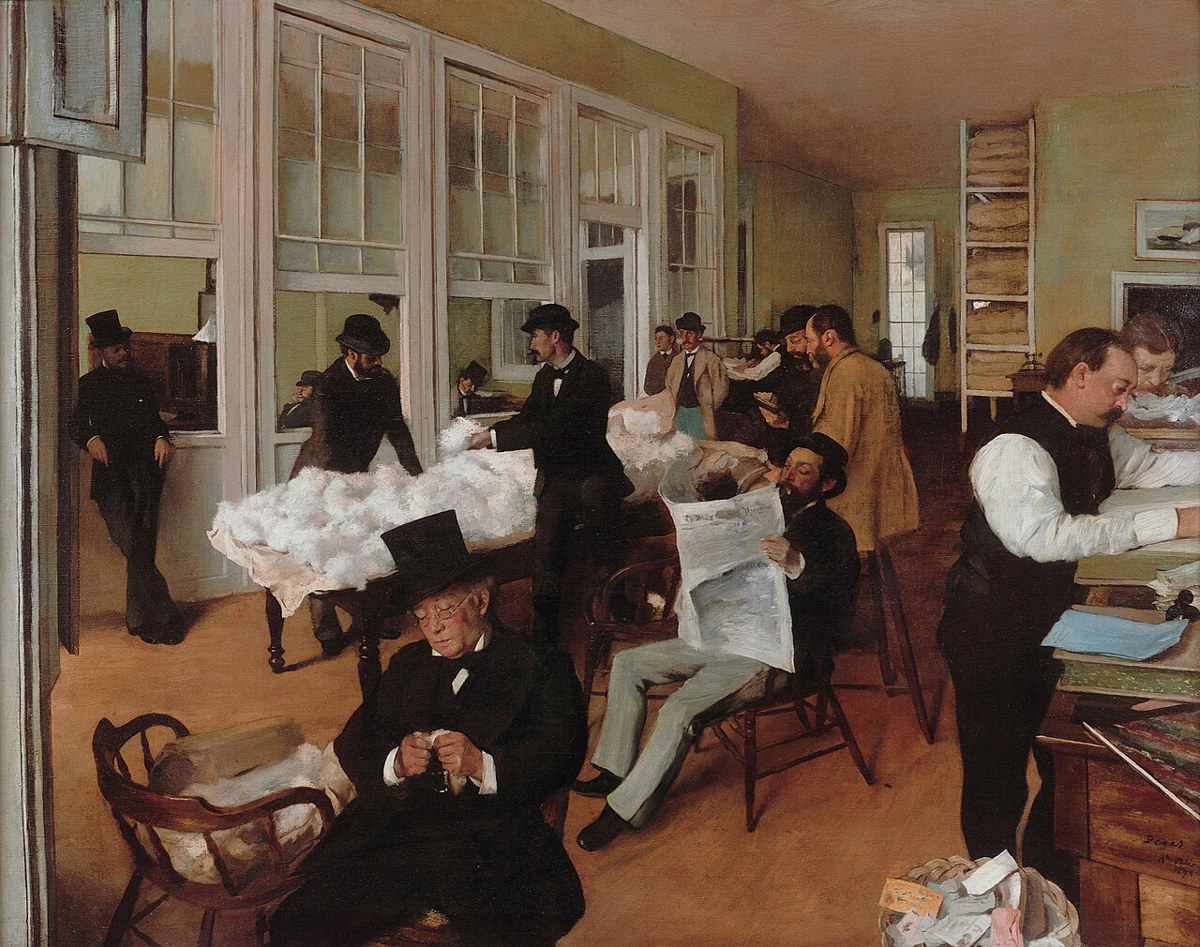
\includegraphics[height=0.42\textheight]{ch3_cotton_office.jpg}\\[1mm]
\imgcap{Edgar Degas, Un birou de bumbac din New Orleans (1873)}
\imgcredit{https://commons.wikimedia.org/wiki/File:Edgar_Germain_Hilaire_Degas_016.jpg}{Imagine: Edgar Degas (1873); domeniu public; Wikimedia Commons}
\end{column}
\end{columns}
\end{frame}

\begin{frame}{Observația lui Mandelbrot}
\itemsize{\small}
\begin{columns}[T]
\begin{column}{0.62\textwidth}
\begin{itemize}
    \item \textbf{Prea multe variații mari}: mult mai multe variații mari decît permite distribuția Normală
    \begin{itemize}
        \item varianța de selecție nu se stabiliza pe măsură ce creștea eșantionul
    \end{itemize}
    \item \textbf{Aceeași formă la orice orizont}: variațiile zilnice și cele lunare arătau la fel după rescalare
    \begin{itemize}
        \item o sumă de multe variații zilnice păstra forma unei singure variații zilnice
    \end{itemize}
    \item \textbf{Propunerea lui}: legi stabile de tip Pareto, cu $\alpha \approx 1{,}7$ \refMandelbrot
    \begin{itemize}
        \item „de tip Pareto”: cozile scad ca o putere a lui $x$, ca în legea veniturilor a lui Pareto
        \item consecință: varianța variațiilor de preț ar fi infinită
    \end{itemize}
\end{itemize}
\end{column}
\begin{column}{0.34\textwidth}
\centering

\includegraphics[height=0.45\textheight]{ch3_mandelbrot.jpg}\\[1mm]
\imgcap{Benoit Mandelbrot (1924--2010)}
\imgcredit{https://commons.wikimedia.org/wiki/File:Benoit_Mandelbrot_mg_1804-d.jpg}{Foto: Rama (2007); CC BY-SA 2.0 fr; Wikimedia Commons}
\end{column}
\end{columns}
\end{frame}

\begin{frame}{Fama testează ideea pe acțiuni}
\itemsize{\small}
\begin{columns}[T]
\begin{column}{0.62\textwidth}
\begin{itemize}
    \item \refFama: randamentele zilnice ale celor 30 de acțiuni din Dow Jones Industrial Average
    \begin{itemize}
        \item mai multe randamente mari decît permite distribuția Normală, pentru fiecare acțiune
        \item estimări ale lui $\alpha$ sub 2: sprijin pentru ipoteza lui Mandelbrot
    \end{itemize}
    \item Au urmat metode de estimare pentru legile stabile simetrice
    \begin{itemize}
        \item \refFamaRoll, \refFamaRollB: estimări pe baza cuantilelor și tabele
    \end{itemize}
    \item În mai puțin de zece ani, dovezile au început să se schimbe: vedeți critica de la finalul capitolului
\end{itemize}
\end{column}
\begin{column}{0.34\textwidth}
\centering

\includegraphics[height=0.45\textheight]{ch3_fama.jpg}\\[1mm]
\imgcap{Eugene Fama la ceremonia Premiului Nobel, 2013}
\imgcredit{https://commons.wikimedia.org/wiki/File:Eugene_Fama_at_Nobel_Prize,_2013.jpg}{Foto: Bengt Nyman (2013); CC BY 2.0; Wikimedia Commons}
\end{column}
\end{columns}
\end{frame}

\begin{frame}{Importanța legii unei sume}
\itemsize{\small}
\begin{itemize}
    \item Un randament logaritmic lunar este suma a circa 21 de randamente logaritmice zilnice
    \begin{itemize}
        \item un model pentru randamentele zilnice implică un model pentru randamentele săptămînale, lunare și anuale
    \end{itemize}
    \item Distribuția Normală își păstrează forma la adunare (\sfmchlink{https://danpele.github.io/SFM/RO/Cursuri/capitol2_distributii_clasice_fapte_stilizate.pdf}{Capitolul 2})
    \begin{itemize}
        \item dar are cozi subțiri: nu surprinde variațiile zilnice mari
    \end{itemize}
    \item \textbf{Întrebare pentru sală}: distribuția Student-t are cozi groase; este suma a 21 de variabile Student-t independente tot Student-t?
    \item \textbf{Răspuns}
    \begin{itemize}
        \item nu: familia Student-t nu este închisă la adunare
        \item dacă varianța ei este finită, suma se apropie de distribuția Normală (teorema limită centrală)
    \end{itemize}
    \item \textbf{Obiectivul}: identificarea tuturor legilor ale căror sume își păstrează forma
\end{itemize}
\end{frame}


%=============================================================================
\section{Stabilitatea la adunare}
%=============================================================================

\begin{frame}{Definiție: legile stabile}
\itemsize{\small}
\begin{itemize}
    \item $X$ este \textbf{stabilă} dacă, pentru $X_1, X_2$ copii independente ale lui $X$ și orice $a, b > 0$, există $c > 0$ și $d$ astfel încît
    \begin{itemize}
        \item $aX_1 + bX_2 \overset{d}{=} cX + d$, unde $\overset{d}{=}$ înseamnă „are aceeași distribuție ca”
        \item $a, b$: ponderile celor două copii; $c$: scala și $d$: deplasarea rezultatului
        \item \textbf{strict stabilă} dacă $d = 0$ pentru orice $a, b$
    \end{itemize}
    \item Altfel spus: o sumă ponderată a două copii are aceeași formă ca o copie
    \begin{itemize}
        \item se schimbă doar scala ($c$) și poziția ($d$)
    \end{itemize}
    \item Prin inducție, pentru $n$ copii independente: $X_1 + \dots + X_n \overset{d}{=} c_n X + d_n$
    \begin{itemize}
        \item singurul factor de scală posibil este $c_n = n^{1/\alpha}$, cu $0 < \alpha \le 2$ \refNolan
    \end{itemize}
    \item $\alpha$ se numește \textbf{indicele de stabilitate} (sau exponentul caracteristic, sau tail index)
\end{itemize}
\end{frame}

\begin{frame}{Două exemple: distribuția Normală și distribuția Cauchy}
\itemsize{\small}
\begin{columns}[T]
\begin{column}{0.64\textwidth}
\begin{itemize}
    \item \textbf{Distribuția Normală}: $X_1, X_2 \sim N(0, \sigma^2)$ independente
    \begin{itemize}
        \item $aX_1 + bX_2 \sim N(0, (a^2 + b^2)\sigma^2)$, deci $c = \sqrt{a^2 + b^2}$
        \item varianțele se adună: $c^2 = a^2 + b^2$, cazul $\alpha = 2$
    \end{itemize}
    \item \textbf{Cauchy}: densitatea $f(x) = \dfrac{1}{\pi(1 + x^2)}$
    \begin{itemize}
        \item $aX_1 + bX_2$ este Cauchy cu scala $c = a + b$
        \item scalele se adună liniar: $c^1 = a^1 + b^1$, cazul $\alpha = 1$
        \item media a $n$ extrageri Cauchy este tot Cauchy standard: medierea nu reduce dispersia
    \end{itemize}
\end{itemize}
\end{column}
\begin{column}{0.32\textwidth}
\centering
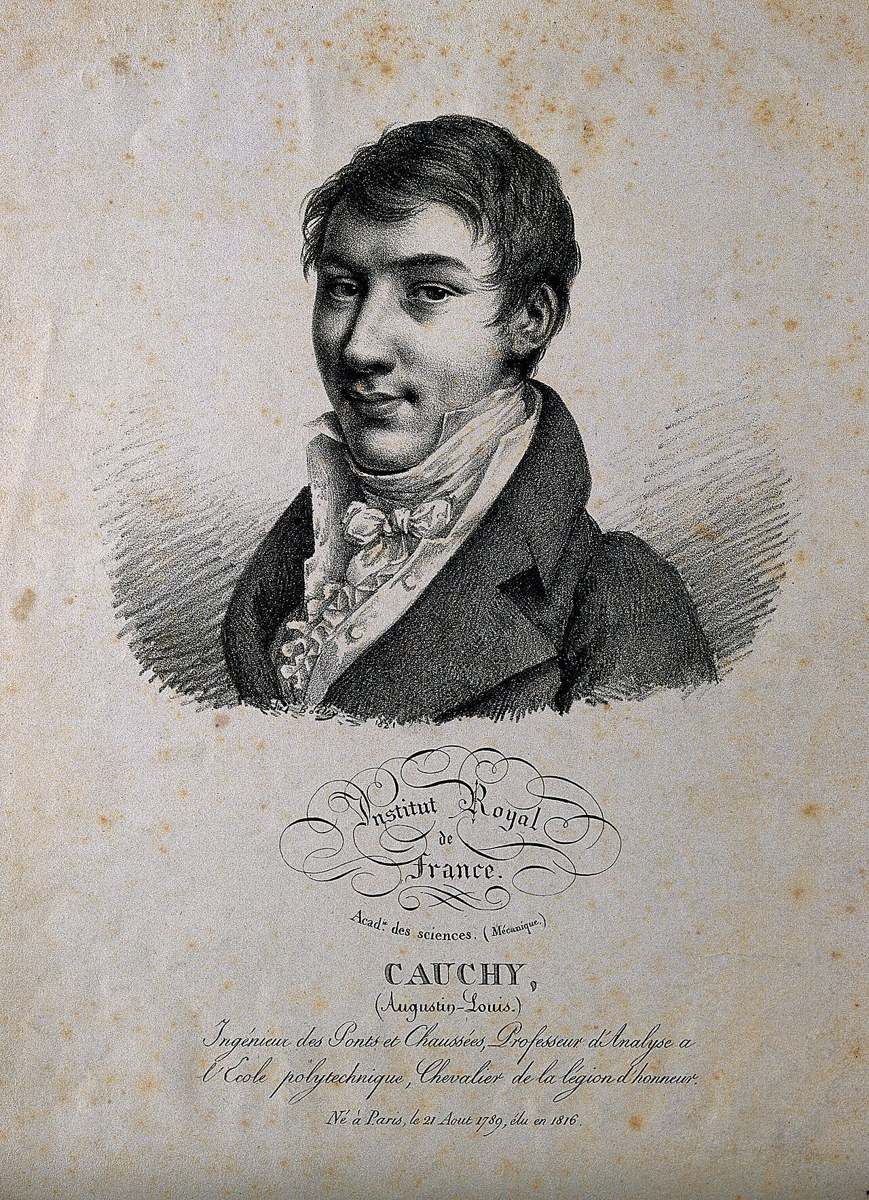
\includegraphics[height=0.46\textheight]{ch3_cauchy.jpg}\\[1mm]
\imgcap{Augustin-Louis Cauchy (1789--1857)}
\imgcredit{https://commons.wikimedia.org/wiki/File:Augstin_Louis,_Baron_Cauchy._Lithograph_by_J._Boilly,_1821._Wellcome_V0001034.jpg}{Litografie: J. Boilly (1821), Wellcome Collection; CC BY 2.0; Wikimedia Commons}
\end{column}
\end{columns}
\end{frame}

\begin{frame}{Regula generală și un exemplu lucrat}
\itemsize{\small}
\begin{itemize}
    \item Pentru $X_1, X_2$ copii independente ale unei $X$ strict stabile cu indicele $\alpha$:
    \begin{itemize}
        \item $c^\alpha = a^\alpha + b^\alpha$, adică $c = (a^\alpha + b^\alpha)^{1/\alpha}$
    \end{itemize}
    \item \textbf{Exemplu}: $a = 3$, $b = 4$
    \begin{itemize}
        \item $\alpha = 2$: $c = \sqrt{9 + 16} = 5{,}00$
        \item $\alpha = 1{,}5$: $c = (3^{1{,}5} + 4^{1{,}5})^{1/1{,}5} = 5{,}58$
        \item $\alpha = 1$: $c = 3 + 4 = 7{,}00$
    \end{itemize}
    \item Cu cît $\alpha$ este mai mic, cu atît scala sumei este mai mare: un singur termen mare poate domina suma
    \item \textbf{Ce credeți?} Pentru $\alpha = 1{,}5$, care este factorul de scală al sumei a două copii?
    \item \textbf{Răspuns}
    \begin{itemize}
        \item $c_2 = 2^{1/1{,}5} = 2^{2/3} = 1{,}59$, mai mare decît $\sqrt{2} \approx 1{,}41$ pentru distribuția Normală
    \end{itemize}
\end{itemize}
\end{frame}

\begin{frame}{Stabilitatea într-o simulare}
\itemsize{\footnotesize}
\begin{center}
    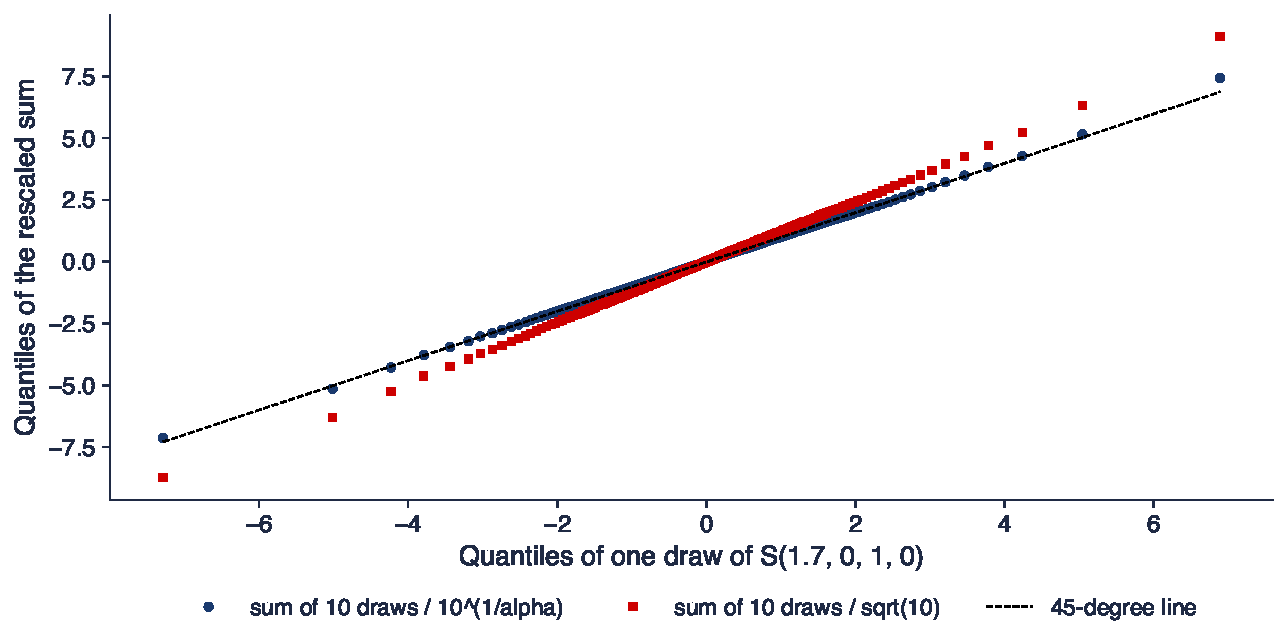
\includegraphics[width=0.97\textwidth,height=0.64\textheight,keepaspectratio]{sfm_ch3_stability_qq.pdf}
\end{center}
\vspace{-0.25cm}
\begin{itemize}
    \item Notație (secțiunea 4): $S(\alpha; \beta; \gamma; \delta)$ este legea stabilă cu indicele $\alpha$, asimetria $\beta$, scala $\gamma$ și poziția $\delta$
    \item Albastru: sumele a 10 extrageri din $S(1{,}7; 0; 1; 0)$ împărțite la $10^{1/1{,}7} = 3{,}87$ se află pe prima bisectoare: aceeași lege ca o singură extragere
    \item Roșu: împărțirea la $\sqrt{10} = 3{,}16$ (regula distribuției Normale) lasă cozile prea largi: cuantila de 99\% este $6{,}31$, față de $5{,}04$
\end{itemize}
\quantlet{SFM\_ch3\_stability\_gclt}{\qlurl{SFM_ch3_stability_gclt}}
\end{frame}

\begin{frame}{Consecințe: orizonturi și diversificare}
\itemsize{\small}
\begin{itemize}
    \item \textbf{Orizontul}: dacă randamentele zilnice sînt i.i.d.\ (independente și identic distribuite) $S(\alpha; 0; \gamma; 0)$, suma pe 20 de zile are scala $20^{1/\alpha}\gamma$
    \begin{itemize}
        \item $\alpha = 2$: $4{,}47\,\gamma$ (regula rădăcinii pătrate a timpului); $\alpha = 1{,}7$: $5{,}83\,\gamma$; $\alpha = 1{,}5$: $7{,}37\,\gamma$
        \item cu $\alpha < 2$, riscul pe orizonturi lungi crește mai repede decît $\sqrt{n}$
    \end{itemize}
    \item \textbf{Diversificarea}: un portofoliu cu ponderi egale din $N$ active stabile i.i.d.\ are scala $N^{1/\alpha - 1}\gamma$
    \begin{itemize}
        \item $N = 10$: $\alpha = 2$ dă $0{,}32\,\gamma$; $\alpha = 1{,}5$ dă $0{,}46\,\gamma$; $\alpha = 1$ dă $1{,}00\,\gamma$
        \item cu $\alpha = 1$, diversificarea nu reduce deloc scala; \refFama\ a discutat această consecință
    \end{itemize}
\end{itemize}
\end{frame}

\begin{frame}{Recapitulare: stabilitatea}
\itemsize{\small}
\begin{itemize}
    \item Lege stabilă: o sumă de copii independente are aceeași formă, doar rescalată și deplasată
    \item Regula scalei: $c^\alpha = a^\alpha + b^\alpha$; $n$ copii: factorul $n^{1/\alpha}$, $0 < \alpha \le 2$
    \item Normală: $\alpha = 2$; Cauchy: $\alpha = 1$
    \item $\alpha$ mic: riscul crește mai repede cu orizontul, iar diversificarea ajută mai puțin
\end{itemize}
\end{frame}


%=============================================================================
\section{Teorema limită centrală generalizată}
%=============================================================================

\begin{frame}{De la CLT clasică la cea generalizată}
\itemsize{\small}
\begin{itemize}
    \item \textbf{CLT clasică} (teorema limită centrală, \sfmchlink{https://danpele.github.io/SFM/RO/Cursuri/capitol2_distributii_clasice_fapte_stilizate.pdf}{Capitolul 2}): $X_i$ i.i.d.\ cu media $\mu$ și varianța finită $\sigma^2$
    \begin{itemize}
        \item $\dfrac{X_1 + \dots + X_n - n\mu}{\sigma\sqrt{n}} \to N(0, 1)$ în distribuție
    \end{itemize}
    \item Ce se întîmplă dacă varianța este infinită? Normalizarea cu $\sqrt{n}$ nu mai este potrivită
    \item \textbf{GCLT} (teorema limită centrală generalizată) \refGK: dacă $(X_1 + \dots + X_n - b_n)/a_n$ converge către o lege nedegenerată, acea lege este stabilă
    \begin{itemize}
        \item $a_n > 0$, $b_n$: constante de normalizare care rescalează și recentrează suma (pentru CLT clasică, $a_n = \sigma\sqrt{n}$, $b_n = n\mu$)
        \item legile stabile sînt \textbf{singurele} limite posibile ale sumelor normalizate de variabile i.i.d.
        \item distribuția Normală este cazul particular $\alpha = 2$
    \end{itemize}
\end{itemize}
\end{frame}

\begin{frame}{Domenii de atracție}
\itemsize{\small}
\begin{columns}[T]
\begin{column}{0.64\textwidth}
\begin{itemize}
    \item \textbf{Domeniul de atracție} al unei legi stabile: toate legile ale căror sume normalizate converg către ea
    \begin{itemize}
        \item varianță finită: domeniul de atracție al distribuției Normale, $a_n \propto \sqrt{n}$
        \item cozi de tip putere $P(|X| > x) \approx C x^{-\alpha}$ cu $0 < \alpha < 2$: legea stabilă cu același $\alpha$, $a_n \propto n^{1/\alpha}$
        \item $C > 0$: o constantă; $\propto$: proporțional cu
    \end{itemize}
    \item Prin urmare, \textbf{coada} distribuției unui randament determină legea sumelor cu mulți termeni
    \item Paul Lévy a caracterizat legile stabile în anii 1920; teoria completă se găsește în \refGK
\end{itemize}
\end{column}
\begin{column}{0.32\textwidth}
\centering
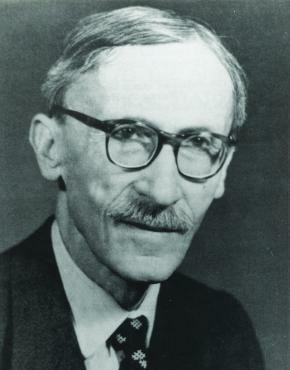
\includegraphics[height=0.42\textheight]{ch3_levy.jpg}\\[1mm]
\imgcap{Paul Lévy (1886--1971)}
\imgcredit{https://commons.wikimedia.org/wiki/File:Paul_Pierre_Levy_1886-1971.jpg}{Foto: Konrad Jacobs, Oberwolfach Photo Collection; CC BY-SA 2.0 de; Wikimedia Commons}
\end{column}
\end{columns}
\end{frame}

\begin{frame}{GCLT într-o simulare}
\itemsize{\footnotesize}
\begin{center}
    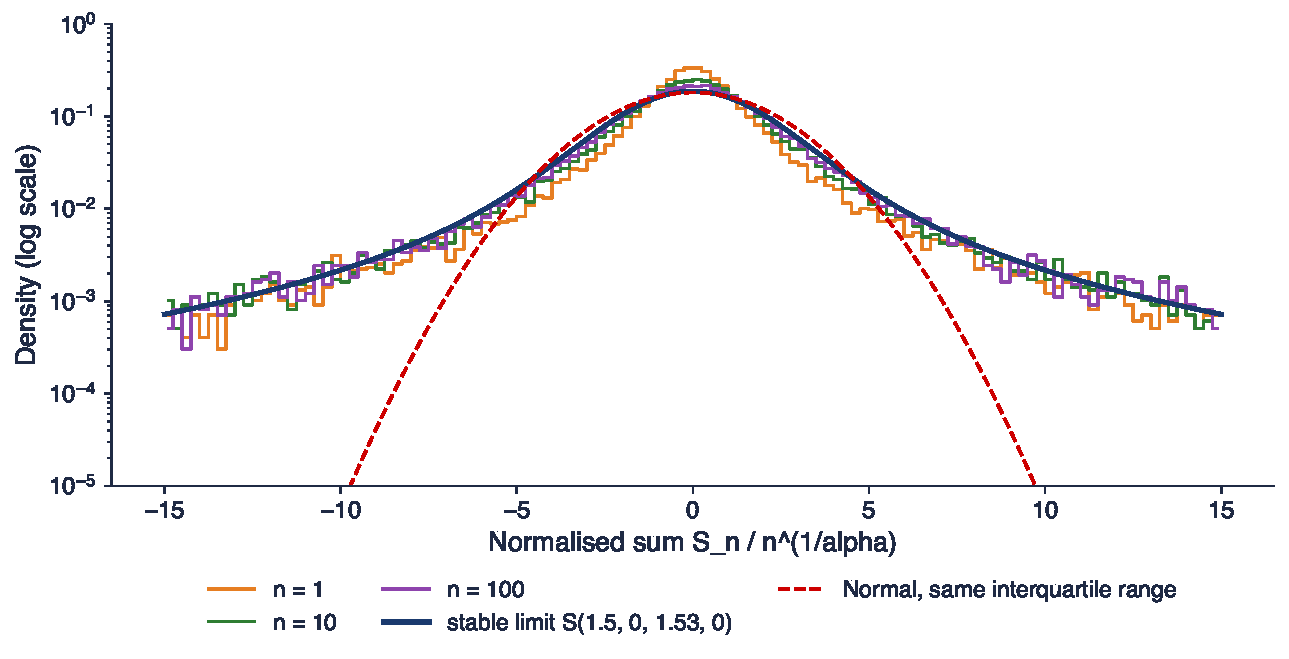
\includegraphics[width=0.97\textwidth,height=0.64\textheight,keepaspectratio]{sfm_ch3_gclt.pdf}
\end{center}
\vspace{-0.25cm}
\begin{itemize}
    \item Student-t cu $\nu = 1{,}5$ grade de libertate: varianță infinită, cozi $\propto x^{-1{,}5}$; sumele a $n$ extrageri împărțite la $n^{1/1{,}5}$
    \item $n = 1, 10, 100$: histogramele se apropie de limita stabilă $S(1{,}5; 0; 1{,}53; 0)$; $P(|\cdot| > 10)$: $2{,}73\%$ pentru $n = 100$, $2{,}64\%$ la limită
    \item O distribuție Normală cu același interval intercuartilic dă $0{,}0005\%$: nu surprinde deloc cozile
\end{itemize}
\quantlet{SFM\_ch3\_stability\_gclt}{\qlurl{SFM_ch3_stability_gclt}}
\end{frame}

\begin{frame}{Implicațiile GCLT pentru randamente}
\itemsize{\small}
\begin{itemize}
    \item Două lumi posibile pentru randamentele zilnice
    \begin{itemize}
        \item \textbf{tail index sub 2} (varianță infinită): randamentele lunare sînt stabile cu \textbf{același} $\alpha$
        \item \textbf{tail index peste 2} (varianță finită): randamentele lunare se apropie de distribuția Normală
    \end{itemize}
    \item Cele două lumi conduc la predicții diferite și testabile despre randamentele pe orizonturi mai lungi
    \item \textbf{Întrebare pentru sală}: căreia dintre cele două lumi îi aparțin randamentele S\&P 500?
    \item \textbf{Răspuns}
    \begin{itemize}
        \item o testăm cu date reale în ultimele secțiuni: estimări ale lui $\alpha$ la orizont zilnic, săptămînal și lunar
    \end{itemize}
\end{itemize}
\end{frame}

\begin{frame}{Recapitulare: teorema limită centrală generalizată}
\itemsize{\small}
\begin{itemize}
    \item CLT clasică: varianță finită, normalizare $\sqrt{n}$, limită Normală
    \item GCLT: legile stabile sînt singurele limite ale sumelor normalizate
    \item Cozi de tip putere cu indicele $\alpha < 2$: normalizare $n^{1/\alpha}$, limită stabilă cu același $\alpha$
    \item Coada distribuției unui singur randament determină legea sumelor cu mulți termeni
\end{itemize}
\end{frame}


%=============================================================================
\section{Parametrii și funcția caracteristică}
%=============================================================================

\begin{frame}{Funcția caracteristică}
\itemsize{\small}
\begin{itemize}
    \item \textbf{Funcția caracteristică} a lui $X$: $\varphi_X(t) = E[e^{itX}] = E[\cos(tX)] + i\,E[\sin(tX)]$, $t \in \mathbb{R}$
    \begin{itemize}
        \item $i = \sqrt{-1}$: unitatea imaginară; $t$: un argument real, nu timpul
        \item există întotdeauna, pentru că $|e^{itX}| = 1$, chiar și cînd nu există niciun moment
        \item determină distribuția în mod unic
    \end{itemize}
    \item Două proprietăți folosite în capitol
    \begin{itemize}
        \item $X, Y$ independente: $\varphi_{X+Y}(t) = \varphi_X(t)\,\varphi_Y(t)$: sumele devin produse
        \item $\varphi_{aX+b}(t) = e^{ibt}\varphi_X(at)$
    \end{itemize}
    \item Normală $N(\mu, \sigma^2)$: $\varphi(t) = \exp(i\mu t - \sigma^2 t^2/2)$
    \item Utilitatea ei: cu excepția a trei cazuri, legile stabile \textbf{nu au densitate în formă închisă}; sînt definite prin $\varphi$
\end{itemize}
\end{frame}

\begin{frame}{Funcția caracteristică stabilă (S1)}
\itemsize{\small}
\begin{itemize}
    \item $X \sim S(\alpha; \beta; \gamma; \delta \mid 1)$ dacă, pentru $\alpha \ne 1$, \refST, \refNolan:
    \begin{itemize}
        \item $\varphi(t) = \exp\Big\{-\gamma^\alpha |t|^\alpha \big[1 - i\beta\,\mathrm{sign}(t)\tan\frac{\pi\alpha}{2}\big] + i\delta t\Big\}$
        \item pentru $\alpha = 1$: $\varphi(t) = \exp\Big\{-\gamma |t| \big[1 + i\beta\,\frac{2}{\pi}\mathrm{sign}(t)\ln|t|\big] + i\delta t\Big\}$
    \end{itemize}
    \item Cei patru parametri
    \begin{itemize}
        \item $\alpha \in (0, 2]$: \textbf{indicele de stabilitate}; $\alpha$ mai mic, cozi mai groase
        \item $\beta \in [-1, 1]$: \textbf{asimetria}; $\beta > 0$ coada dreaptă mai groasă, $\beta < 0$ coada stîngă mai groasă
        \item $\gamma > 0$: \textbf{scala} (joacă rolul lui $\sigma$); $\delta \in \mathbb{R}$: \textbf{poziția}
    \end{itemize}
    \item $\mathrm{sign}(t)$: $+1$ pentru $t > 0$, $-1$ pentru $t < 0$; termenul cu $\beta$ face legea asimetrică
    \item Stabilitatea este vizibilă: $\varphi(t)^n$ are aceeași formă, cu $\gamma^\alpha$ înlocuit de $n\gamma^\alpha$
\end{itemize}
\end{frame}

\begin{frame}{Efectul lui $\alpha$}
\itemsize{\footnotesize}
\begin{center}
    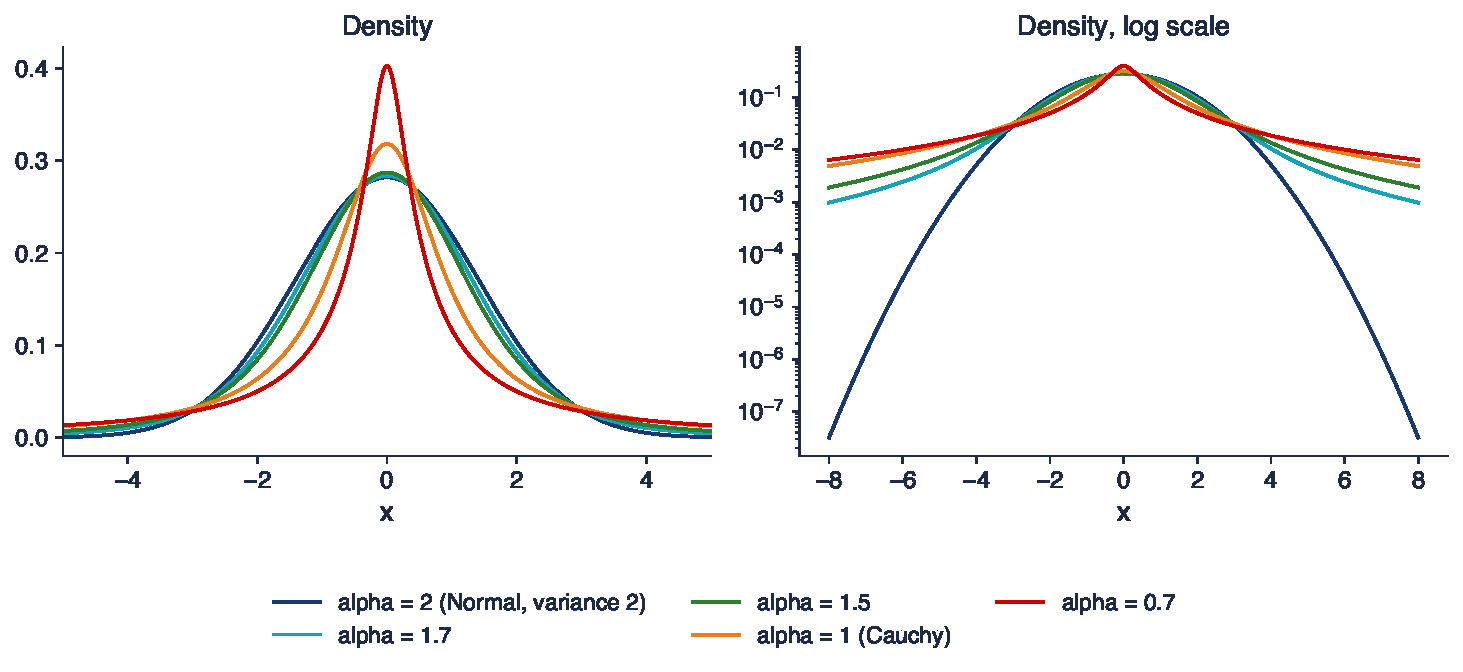
\includegraphics[width=0.97\textwidth,height=0.64\textheight,keepaspectratio]{sfm_ch3_density_alpha.pdf}
\end{center}
\vspace{-0.25cm}
\begin{itemize}
    \item Legi simetrice $S(\alpha; 0; 1; 0)$: $\alpha$ mai mic dă un vîrf mai înalt și mai îngust și cozi mult mai groase
    \item Scara logaritmică: coada distribuției Normale ($\alpha = 2$) scade ca $e^{-x^2/4}$; celelalte scad ca o putere a lui $x$
\end{itemize}
\quantlet{SFM\_ch3\_densities}{\qlurl{SFM_ch3_densities}}
\end{frame}

\begin{frame}{Efectul lui $\beta$ și $\gamma$}
\itemsize{\footnotesize}
\begin{center}
    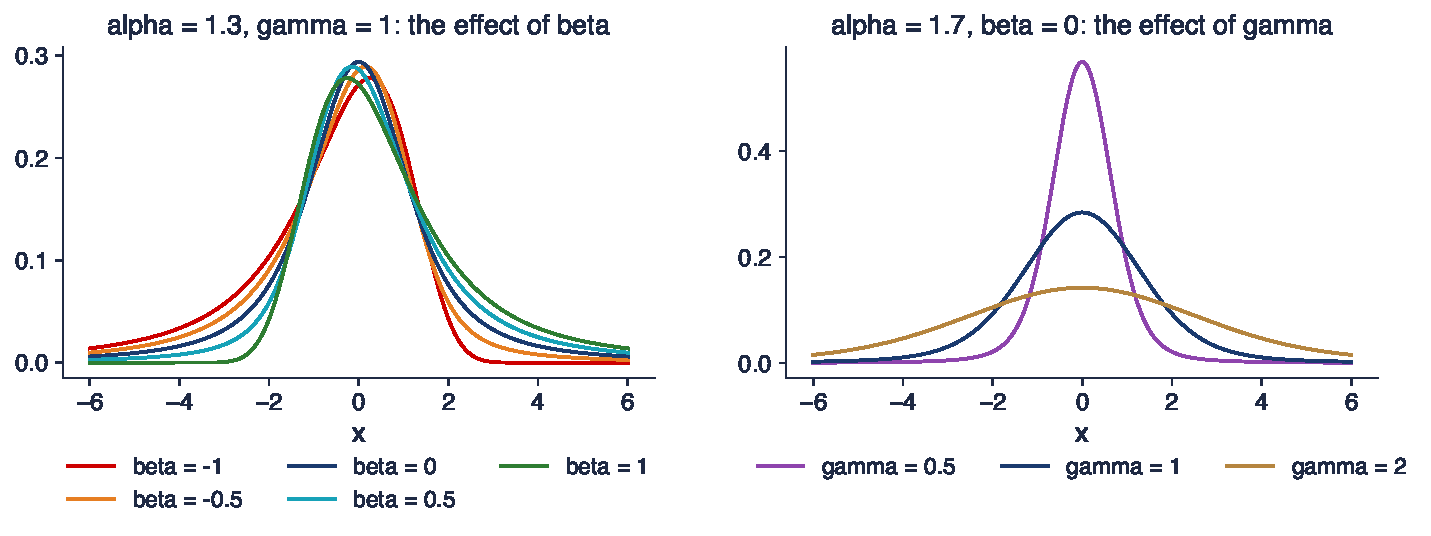
\includegraphics[width=0.97\textwidth,height=0.64\textheight,keepaspectratio]{sfm_ch3_density_beta.pdf}
\end{center}
\vspace{-0.25cm}
\begin{itemize}
    \item $\beta$ redistribuie masa între cozi: $\beta = 1$ (verde) are coada dreaptă mai groasă, $\beta = -1$ (roșu) coada stîngă mai groasă
    \item $\gamma$ întinde densitatea: dublarea lui $\gamma$ dublează fiecare cuantilă în jurul lui $\delta$
\end{itemize}
\quantlet{SFM\_ch3\_densities}{\qlurl{SFM_ch3_densities}}
\end{frame}

\begin{frame}{Două parametrizări: S0 și S1}
\itemsize{\small}
\begin{itemize}
    \item \textbf{S0} (recomandarea lui Nolan pentru analiza datelor), $\alpha \ne 1$:
    \begin{itemize}
        \item $\varphi(t) = \exp\Big\{-\gamma^\alpha |t|^\alpha \big[1 + i\beta\,\mathrm{sign}(t)\tan\frac{\pi\alpha}{2}\big(|\gamma t|^{1-\alpha} - 1\big)\big] + i\delta_0 t\Big\}$
    \end{itemize}
    \item Diferă doar poziția: $\delta_0 = \delta_1 + \beta\gamma\tan\frac{\pi\alpha}{2}$ ($\alpha \ne 1$)
    \begin{itemize}
        \item $\delta_0$, $\delta_1$: parametrul de poziție în S0 și în S1; $\alpha$, $\beta$ și $\gamma$ sînt aceleași în ambele
        \item pentru $\beta = 0$ cele două coincid
    \end{itemize}
    \item Rolul fiecăreia
    \begin{itemize}
        \item S1: algebră mai simplă pentru sume; folosită în majoritatea cărților de teorie \refST
        \item S0: densitatea se schimbă continuu cu $\alpha$ și $\beta$; mai bună pentru estimare și grafice \refNolan
    \end{itemize}
\end{itemize}
\end{frame}

\begin{frame}{S1 și S0 în apropiere de $\alpha = 1$}
\itemsize{\footnotesize}
\begin{center}
    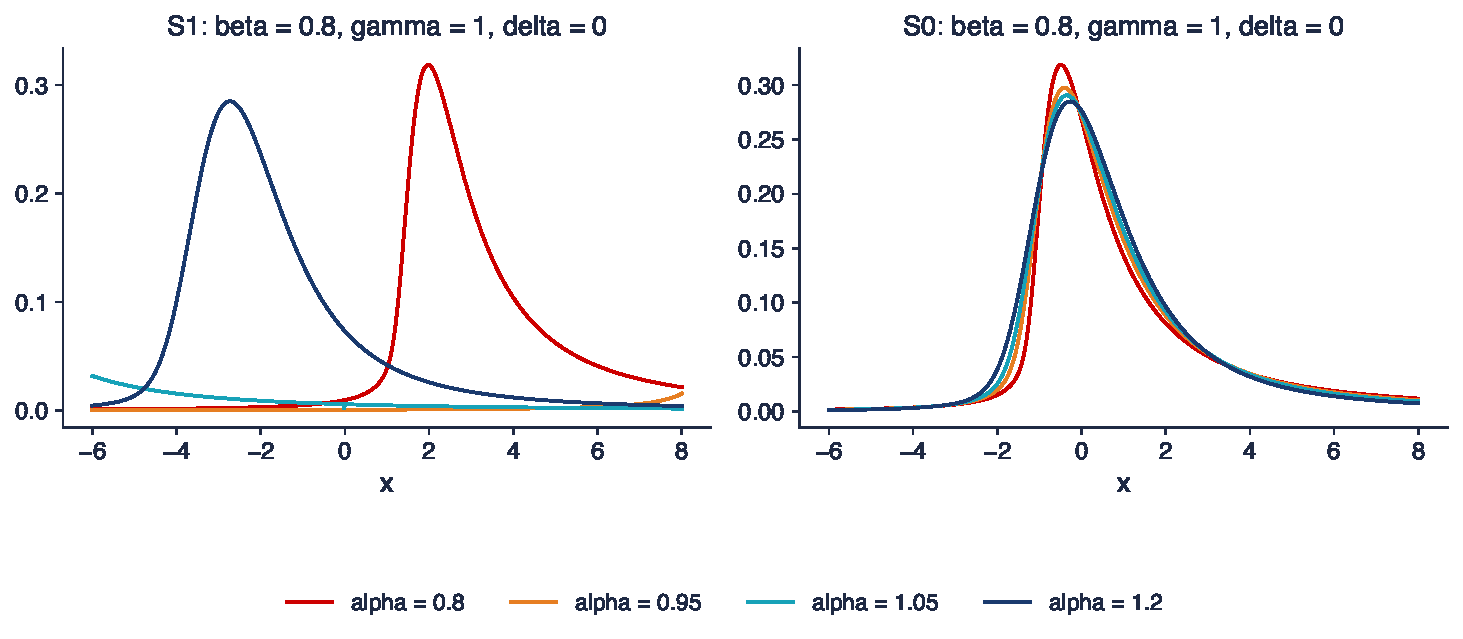
\includegraphics[width=0.97\textwidth,height=0.64\textheight,keepaspectratio]{sfm_ch3_s0_s1.pdf}
\end{center}
\vspace{-0.25cm}
\begin{itemize}
    \item S1 (stînga): cu $\beta = 0{,}8$, densitatea se deplasează spre $+\infty$ cînd $\alpha \uparrow 1$ și revine dinspre $-\infty$ cînd $\alpha \downarrow 1$, pentru că $\tan\frac{\pi\alpha}{2}$ tinde la infinit
    \item S0 (dreapta): aceleași patru legi, deplasate; modul rămîne lîngă 0 și se schimbă lin
\end{itemize}
\quantlet{SFM\_ch3\_densities}{\qlurl{SFM_ch3_densities}}
\end{frame}

\begin{frame}{Atenție la parametrizare în software}
\itemsize{\small}
\begin{itemize}
    \item \texttt{scipy.stats.levy\_stable} folosește implicit \textbf{S1}
    \begin{itemize}
        \item se schimbă cu \texttt{levy\_stable.parameterization = 'S0'}
        \item argumente: \texttt{levy\_stable.pdf(x, alpha, beta, loc=delta, scale=gamma)}
    \end{itemize}
    \item Lucrările și programele raportează $\delta$ în S0, în S1 sau în alte parametrizări: verificați parametrizarea înainte de a compara rezultatele
    \item Capcana scalei: $S(2; 0; \gamma; \delta)$ este $N(\delta, 2\gamma^2)$, nu $N(\delta, \gamma^2)$
    \begin{itemize}
        \item deci $\gamma = \sigma/\sqrt{2}$ pentru distribuția Normală
    \end{itemize}
    \item În acest curs: estimările sînt în S0, iar $\delta_1$ este raportat separat
\end{itemize}
\end{frame}

\begin{frame}{Trei legi cu densitate în formă închisă}
\itemsize{\small}
\begin{itemize}
    \item \textbf{Distribuția Normală}: $\alpha = 2$ ($\beta$ nu are niciun rol)
    \begin{itemize}
        \item $\varphi(t) = \exp(-\gamma^2 t^2 + i\delta t)$, adică $N(\delta, 2\gamma^2)$
    \end{itemize}
    \item \textbf{Cauchy}: $\alpha = 1$, $\beta = 0$
    \begin{itemize}
        \item $f(x) = \dfrac{\gamma}{\pi\,(\gamma^2 + (x - \delta)^2)}$; $\varphi(t) = \exp(-\gamma|t| + i\delta t)$
    \end{itemize}
    \item \textbf{Lévy}: $\alpha = 1/2$, $\beta = 1$ (S1); complet asimetrică la dreapta
    \begin{itemize}
        \item $f(x) = \sqrt{\dfrac{\gamma}{2\pi}}\,(x - \delta)^{-3/2} \exp\Big(-\dfrac{\gamma}{2(x - \delta)}\Big)$ pentru $x > \delta$
        \item momentul în care o mișcare browniană atinge prima dată un nivel are o lege Lévy
    \end{itemize}
    \item Toate celelalte densități stabile se calculează numeric din $\varphi$ \refNolanA, \refMDC
\end{itemize}
\end{frame}

\begin{frame}{Distribuțiile Normală, Cauchy și Lévy}
\itemsize{\footnotesize}
\begin{center}
    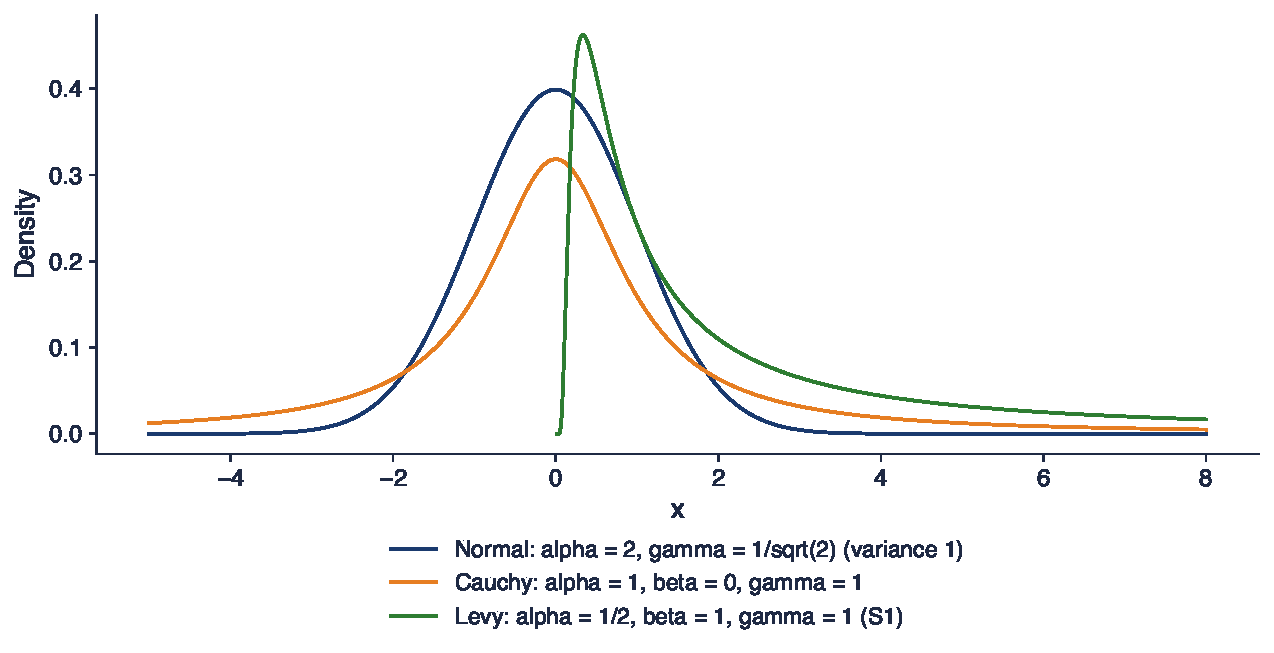
\includegraphics[width=0.97\textwidth,height=0.60\textheight,keepaspectratio]{sfm_ch3_special_cases.pdf}
\end{center}
\vspace{-0.25cm}
\begin{itemize}
    \item Cauchy: vîrf mai jos, cozi mult mai groase decît distribuția Normală cu varianța 1
    \item Lévy: doar valori pozitive, o coadă dreaptă lungă; media ei este infinită
\end{itemize}
\quantlet{SFM\_ch3\_densities}{\qlurl{SFM_ch3_densities}}
\end{frame}

\begin{frame}{Exemplu lucrat: S1 și S0 în $t = 1$}
\itemsize{\small}
\begin{itemize}
    \item $X$ cu $\alpha = 1{,}5$, $\beta = 0{,}3$, $\gamma = 1$, $\delta = 0$; observați că $\tan\frac{3\pi}{4} = -1$
    \item \textbf{S1}: $\ln\varphi(1) = -1\cdot[1 - i \cdot 0{,}3 \cdot (-1)] = -1 - 0{,}3i$
    \begin{itemize}
        \item $\varphi(1) = e^{-1}(\cos 0{,}3 - i \sin 0{,}3) = 0{,}351 - 0{,}109i$; $|\varphi(1)| = e^{-1} = 0{,}368$
    \end{itemize}
    \item \textbf{S0}: factorul $|t|^{1-\alpha} - 1$ este 0 în $t = 1$, deci $\varphi(1) = e^{-1} = 0{,}368$, un număr real
    \begin{itemize}
        \item același modul: cele două legi diferă doar printr-o deplasare
        \item deplasarea $= \beta\gamma\tan\frac{\pi\alpha}{2} = -0{,}3$: legea S1 cu $\delta_1 = 0$ este legea S0 cu $\delta_0 = -0{,}3$
    \end{itemize}
\end{itemize}
\end{frame}

\begin{frame}{Recapitulare: parametrii și funcția caracteristică}
\itemsize{\small}
\begin{itemize}
    \item Legile stabile se definesc prin $\varphi(t)$; densitatea se calculează numeric
    \item $\alpha$ cozi, $\beta$ asimetrie, $\gamma$ scală, $\delta$ poziție
    \item S0 și S1: diferă doar $\delta$, $\delta_0 = \delta_1 + \beta\gamma\tan\frac{\pi\alpha}{2}$; scipy folosește implicit S1
    \item Forme închise: Normală ($\alpha = 2$, varianța $2\gamma^2$), Cauchy, Lévy
\end{itemize}
\end{frame}


%=============================================================================
\section{Cozi și momente}
%=============================================================================

\begin{frame}{Cozi de tip putere}
\itemsize{\small}
\begin{itemize}
    \item Pentru $\alpha < 2$, cînd $x \to \infty$ \refNolan:
    \begin{itemize}
        \item $P(X > x) \sim \gamma^\alpha c_\alpha (1 + \beta)\, x^{-\alpha}$ și $P(X < -x) \sim \gamma^\alpha c_\alpha (1 - \beta)\, x^{-\alpha}$
        \item $c_\alpha = \Gamma(\alpha)\sin(\pi\alpha/2)/\pi$, cu $\Gamma$ funcția gamma; $f \sim g$ înseamnă $f/g \to 1$
    \end{itemize}
    \item Pe axe log-log, coada este o dreaptă cu panta $-\alpha$
    \begin{itemize}
        \item dublarea pragului împarte probabilitatea din coadă la $2^\alpha$: $\times 0{,}31$ pentru $\alpha = 1{,}7$
    \end{itemize}
    \item Coada distribuției Normale scade ca $e^{-x^2/(4\gamma^2)}$: dublarea pragului o face practic nulă
    \item $\beta = \pm 1$ cu $\alpha < 1$: una dintre cozi lipsește (suportul legii este o semidreaptă)
\end{itemize}
\end{frame}

\begin{frame}{Cozile pe axe log-log}
\itemsize{\footnotesize}
\begin{center}
    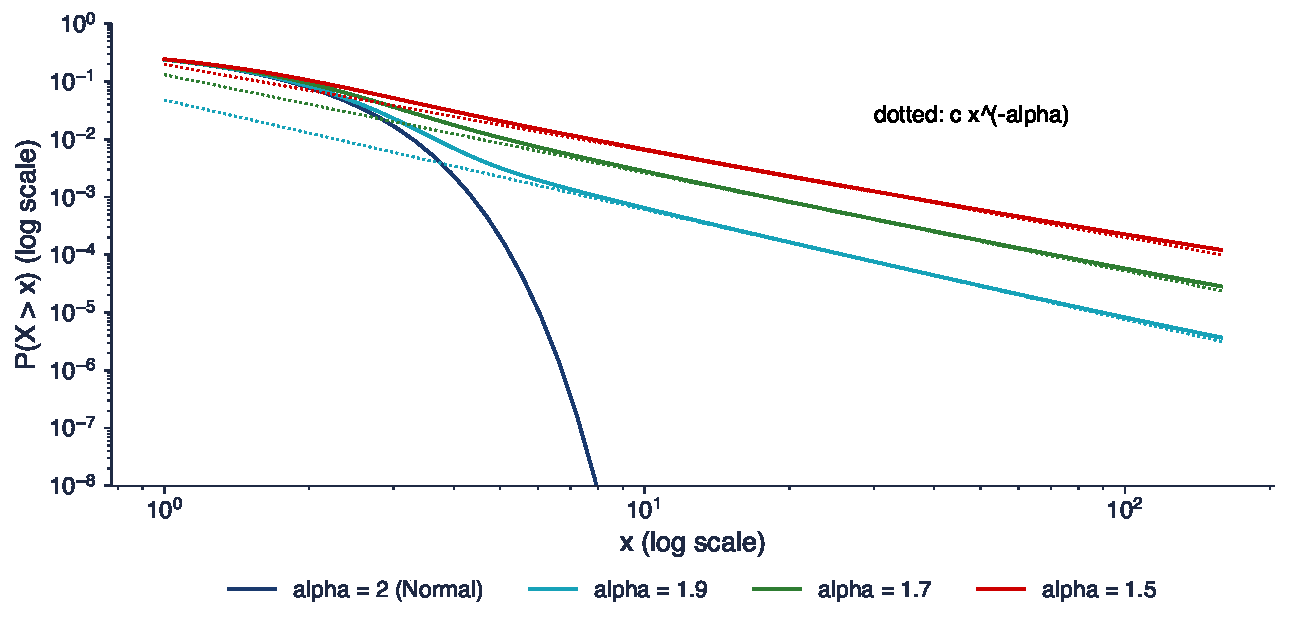
\includegraphics[width=0.97\textwidth,height=0.64\textheight,keepaspectratio]{sfm_ch3_tails_loglog.pdf}
\end{center}
\vspace{-0.25cm}
\begin{itemize}
    \item Linie continuă: $P(X > x)$ pentru $S(\alpha; 0; 1; 0)$; linie punctată: legea de tip putere $c_\alpha x^{-\alpha}$, atinsă deja în jurul lui $x = 5$
    \item $P(X > 10)$: $0{,}279\%$ pentru $\alpha = 1{,}7$, $0{,}667\%$ pentru $\alpha = 1{,}5$, circa $8\times 10^{-11}\%$ pentru distribuția Normală
\end{itemize}
\quantlet{SFM\_ch3\_tails\_moments}{\qlurl{SFM_ch3_tails_moments}}
\end{frame}

\begin{frame}{Existența momentelor}
\itemsize{\small}
\begin{itemize}
    \item Pentru $0 < \alpha < 2$: $E|X|^p < \infty$ dacă și numai dacă $p < \alpha$
    \begin{itemize}
        \item $E|X|^p$: momentul absolut de ordin $p > 0$; $p = 1$ corespunde mediei, $p = 2$ varianței
        \item motivul: $|x|^p$ înmulțit cu o densitate de ordinul $|x|^{-\alpha-1}$ este integrabil doar dacă $p < \alpha$
    \end{itemize}
    \item Consecințe
    \begin{itemize}
        \item $\alpha < 2$: \textbf{varianță infinită}; asimetria și boltirea nu sînt definite
        \item $1 < \alpha < 2$: media există; în S1 este egală cu $\delta_1$
        \item $\alpha \le 1$: nici media nu există (Cauchy, Lévy)
        \item $\alpha = 2$: toate momentele există
    \end{itemize}
    \item \textbf{Ce credeți?} Mandelbrot a găsit $\alpha \approx 1{,}7$ pentru bumbac. Există media variației zilnice?
    \item \textbf{Răspuns}
    \begin{itemize}
        \item da, pentru că $1 < 1{,}7$; dar varianța nu există, pentru că $2 > 1{,}7$
    \end{itemize}
\end{itemize}
\end{frame}

\begin{frame}{Varianța de selecție nu se stabilizează}
\itemsize{\footnotesize}
\begin{center}
    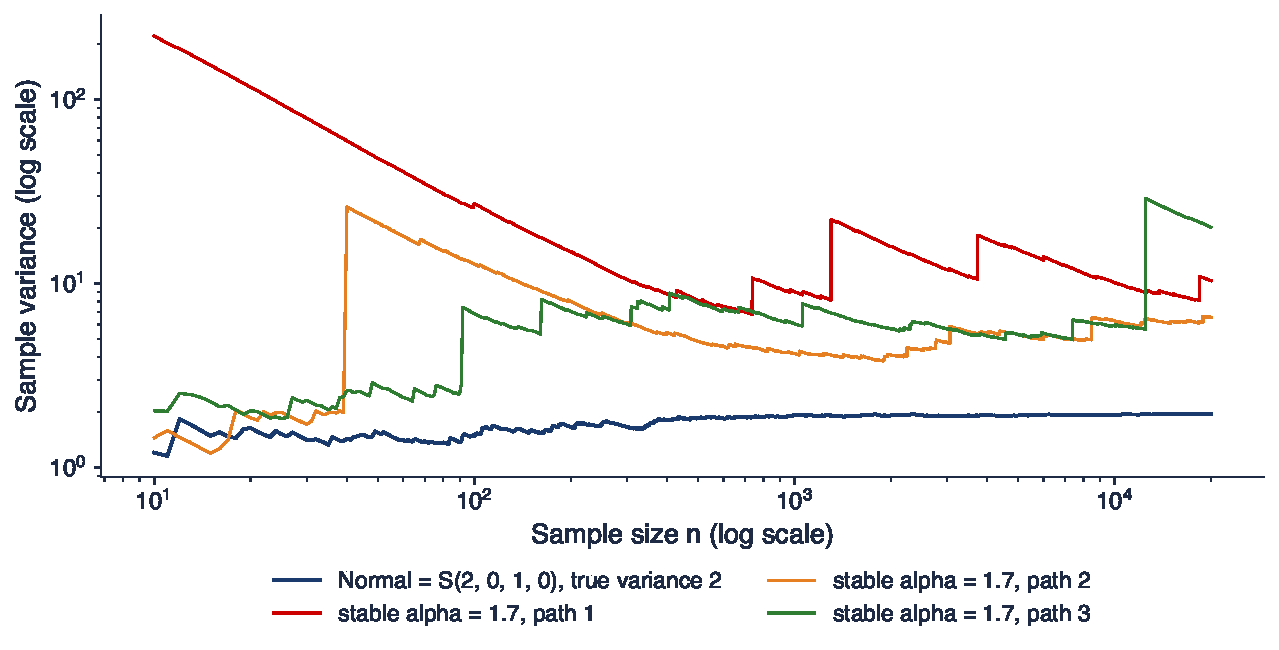
\includegraphics[width=0.97\textwidth,height=0.64\textheight,keepaspectratio]{sfm_ch3_running_var_sim.pdf}
\end{center}
\vspace{-0.25cm}
\begin{itemize}
    \item Distribuția Normală (albastru): varianța de selecție converge la valoarea adevărată 2
    \item Stabilă $\alpha = 1{,}7$: fiecare extragere mare produce un salt al varianței; după 20\,000 de extrageri, cele trei traiectorii ajung la $10{,}4$, $6{,}6$, $20{,}2$
    \item Același fenomen l-a observat Mandelbrot în prețurile bumbacului
\end{itemize}
\quantlet{SFM\_ch3\_tails\_moments}{\qlurl{SFM_ch3_tails_moments}}
\end{frame}

\begin{frame}{Probabilitățile din cozi: distribuția stabilă și distribuția Normală}
\itemsize{\small}
\begin{center}
\footnotesize
\begin{tabular}{rrrr}
\toprule
$k$ & $P(|X| > k)$, Normală \% & $P(|X| > k)$, $\alpha = 1{,}7$ \% & raport \\
\midrule
$2$ & $15{,}73$ & $18{,}59$ & $1{,}2$ \\
$3$ & $3{,}39$ & $7{,}25$ & $2{,}1$ \\
$5$ & $0{,}041$ & $2{,}13$ & $52{,}4$ \\
$10$ & $1{,}5\times 10^{-10}$ & $0{,}56$ & $3{,}6\times 10^{9}$ \\
\bottomrule
\end{tabular}
\end{center}
\begin{itemize}
    \item Ambele legi au $\beta = 0$, $\gamma = 1$, $\delta = 0$; legea Normală este deci $N(0, 2)$
    \item În jurul centrului, cele două legi sînt apropiate; departe în cozi, diferă prin ordine de mărime
    \item Un model de risc se evaluează în cozi, unde alegerea legii contează cel mai mult
\end{itemize}\quantlet{SFM\_ch3\_tails\_moments}{\qlurl{SFM_ch3_tails_moments}}
\end{frame}

\begin{frame}{Varianța infinită și măsurile de risc}
\itemsize{\small}
\begin{itemize}
    \item Instrumente care au nevoie de varianță finită
    \begin{itemize}
        \item volatilitatea, raportul Sharpe și eroarea lui standard (\sfmchlink{https://danpele.github.io/SFM/RO/Cursuri/capitol1_date_randamente_indicatori.pdf}{Capitolul 1}); portofoliile medie--varianță; intervalele de încredere obținute din CLT
        \item cu $\alpha < 2$, aceste mărimi se pot calcula pe orice eșantion, dar nu estimează nimic
    \end{itemize}
    \item Instrumente care rămîn valabile
    \begin{itemize}
        \item cuantilele există întotdeauna: $\mathrm{VaR}_{1\%} = -q_{1\%}$, pierderea depășită cu probabilitatea 1\%
        \item $\mathrm{ES}_{2{,}5\%}$ (expected shortfall, pierderea medie dincolo de VaR) există doar dacă $\alpha > 1$
        \item scala $\gamma$ și intervalul intercuartilic înlocuiesc abaterea standard
    \end{itemize}
    \item VaR și ES sînt tratate pe larg în \sfmchlink{https://danpele.github.io/SFM/RO/Cursuri/capitol10_var_es_backtesting.pdf}{Capitolul 10}
\end{itemize}
\end{frame}

\begin{frame}{Recapitulare: cozi și momente}
\itemsize{\small}
\begin{itemize}
    \item Cozi: $P(|X| > x) \propto x^{-\alpha}$; o dreaptă pe axe log-log
    \item Momente: $E|X|^p < \infty$ dacă și numai dacă $p < \alpha$; $\alpha < 2$ înseamnă varianță infinită
    \item Varianța de selecție a unui eșantion stabil are salturi și nu se stabilizează
    \item Cuantilele, VaR și scala $\gamma$ își păstrează sensul
\end{itemize}
\end{frame}


%=============================================================================
\section{Simulare}
%=============================================================================

\begin{frame}{Metoda Chambers--Mallows--Stuck (cazul simetric)}
\itemsize{\small}
\begin{itemize}
    \item Nu există densitate în formă închisă, dar variabilele stabile se simulează ușor \refCMS
    \item \textbf{CMS} (Chambers--Mallows--Stuck) pentru $S(\alpha; 0; 1; 0)$:
    \begin{itemize}
        \item extrageți $V \sim U(-\pi/2, \pi/2)$, un unghi uniform, și $W \sim \mathrm{Exp}(1)$, o variabilă exponențială cu media 1, independente
        \item $X = \dfrac{\sin(\alpha V)}{(\cos V)^{1/\alpha}} \left(\dfrac{\cos((1 - \alpha)V)}{W}\right)^{(1 - \alpha)/\alpha}$
        \item apoi $\gamma X + \delta \sim S(\alpha; 0; \gamma; \delta)$
    \end{itemize}
    \item Verificări pe cazuri particulare
    \begin{itemize}
        \item $\alpha = 1$: $X = \tan V$, o variabilă Cauchy
        \item $\alpha = 2$: $X = 2\sin V\sqrt{W}$, o variabilă $N(0, 2)$
    \end{itemize}
\end{itemize}
\end{frame}

\begin{frame}{Cazul general ($\beta \ne 0$)}
\itemsize{\small}
\begin{itemize}
    \item Pentru $\alpha \ne 1$, parametrizarea S1 \refWeron:
    \begin{itemize}
        \item $B = \dfrac{\arctan(\beta\tan\frac{\pi\alpha}{2})}{\alpha}$, \quad $S = \Big(1 + \beta^2\tan^2\frac{\pi\alpha}{2}\Big)^{1/(2\alpha)}$
        \item $X = S\,\dfrac{\sin(\alpha(V + B))}{(\cos V)^{1/\alpha}} \left(\dfrac{\cos(V - \alpha(V + B))}{W}\right)^{(1 - \alpha)/\alpha} \sim S(\alpha; \beta; 1; 0 \mid 1)$
    \end{itemize}
    \item $B$, $S$: constante auxiliare care depind doar de $\alpha$ și $\beta$; pentru $\beta = 0$, $B = 0$ și $S = 1$
    \item De la extragerea standard la orice parametri
    \begin{itemize}
        \item S1: $\gamma X + \delta_1$; S0: $\gamma X + \delta_0 - \beta\gamma\tan\frac{\pi\alpha}{2}$
    \end{itemize}
    \item Weron (1996) a corectat o formulă din lucrarea originală pentru $\beta \ne 0$; \texttt{scipy.stats.levy\_stable.rvs} folosește aceeași metodă
\end{itemize}
\end{frame}

\begin{frame}{Exemplu lucrat: o extragere pas cu pas}
\itemsize{\small}
\begin{itemize}
    \item $\alpha = 1{,}5$, $\beta = 0$; o extragere uniformă $U = 0{,}8$ și o extragere exponențială $W = 1{,}2$
    \item Pași
    \begin{itemize}
        \item $V = \pi(U - 1/2) = 0{,}942$: transformă $U$, uniformă pe $(0, 1)$, într-un unghi uniform pe $(-\pi/2, \pi/2)$
        \item $\sin(\alpha V) = 0{,}988$; $(\cos V)^{1/\alpha} = 0{,}702$
        \item $\big(\cos((1 - \alpha)V)/W\big)^{(1 - \alpha)/\alpha} = 1{,}104$
        \item $X = 0{,}988/0{,}702 \times 1{,}104 = 1{,}554$
    \end{itemize}
    \item Repetați cu noi perechi $(U, W)$ pentru un eșantion de orice mărime
\end{itemize}
\end{frame}

\begin{frame}{Extrageri CMS față de densitatea exactă}
\itemsize{\footnotesize}
\begin{center}
    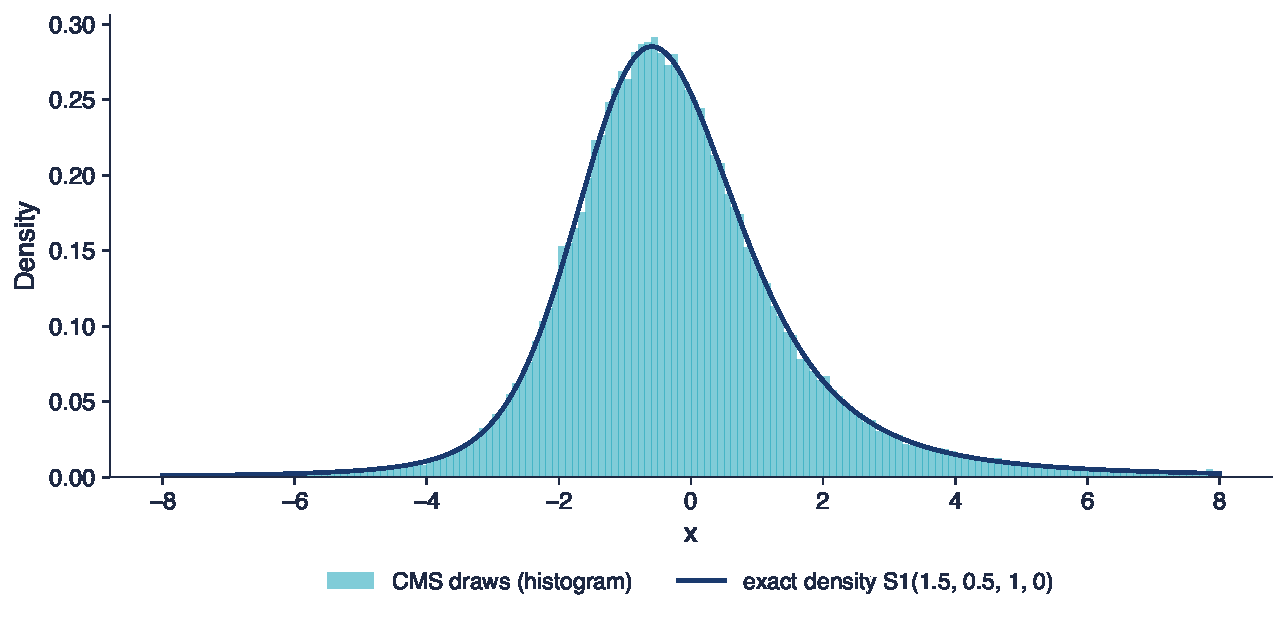
\includegraphics[width=0.97\textwidth,height=0.64\textheight,keepaspectratio]{sfm_ch3_cms.pdf}
\end{center}
\vspace{-0.25cm}
\begin{itemize}
    \item 100\,000 de extrageri CMS din $S(1{,}5; 0{,}5; 1; 0 \mid 1)$: histograma urmează densitatea calculată din $\varphi$
    \item Cuantilele de 1\% și 99\%: eșantion $-5{,}47$ și $9{,}52$, exact $-5{,}40$ și $9{,}76$
    \item Testul KS (Kolmogorov--Smirnov) cu două eșantioane față de \texttt{levy\_stable.rvs}: statistica $0{,}0044$, p-value $0{,}30$, nicio diferență
\end{itemize}
\quantlet{SFM\_ch3\_sim\_stable}{\qlurl{SFM_ch3_sim_stable}}
\end{frame}

\begin{frame}{Recapitulare: simularea}
\itemsize{\small}
\begin{itemize}
    \item CMS: un unghi uniform $V$ și un $W$ exponențial dau o extragere stabilă
    \item Cazurile particulare verifică formula: $\tan V$ (Cauchy), $2\sin V\sqrt{W}$ (Normală)
    \item Cazul asimetric: formula din \refWeron; deplasare cu $\beta\gamma\tan\frac{\pi\alpha}{2}$ pentru S0
\end{itemize}
\end{frame}


%=============================================================================
\section{Estimare}
%=============================================================================

\begin{frame}{Trei familii de estimatori}
\itemsize{\small}
\begin{itemize}
    \item \textbf{Metodele cuantilelor}: potrivesc cuantilele de selecție cu cele ale legii stabile
    \begin{itemize}
        \item \refFamaRollB\ pentru legi simetrice; \refMcCulloch\ pentru toți cei patru parametri
    \end{itemize}
    \item \textbf{Metodele funcției caracteristice}: regresia lui $\ln(-\ln|\hat\varphi(t)|^2)$ empiric pe $\ln|t|$
    \begin{itemize}
        \item $\hat\varphi(t) = \frac1n\sum_{j=1}^n e^{itr_j}$: funcția caracteristică empirică; $|\varphi(t)|^2 = e^{-2\gamma^\alpha|t|^\alpha}$, deci relația dublu logaritmică este liniară în $\ln|t|$
        \item \refKoutrouvelis; panta estimează $\alpha$
    \end{itemize}
    \item \textbf{Verosimilitatea maximă} (ML): cea mai precisă, dacă densitatea poate fi calculată
    \begin{itemize}
        \item \refNolanML, \refMRDC
    \end{itemize}
    \item O implementare SAS a acestor estimatori este descrisă în \refPele
\end{itemize}
\end{frame}

\begin{frame}{Metoda cuantilelor a lui McCulloch}
\itemsize{\small}
\begin{itemize}
    \item Două rapoarte de cuantile de selecție $\hat q_p$, independente de poziție și de scală \refMcCulloch:
    \begin{itemize}
        \item $\nu_\alpha = \dfrac{\hat q_{0{,}95} - \hat q_{0{,}05}}{\hat q_{0{,}75} - \hat q_{0{,}25}}$ (lățimea cozilor față de corp)
        \item $\nu_\beta = \dfrac{\hat q_{0{,}95} + \hat q_{0{,}05} - 2\hat q_{0{,}5}}{\hat q_{0{,}95} - \hat q_{0{,}05}}$ (asimetria)
    \end{itemize}
    \item $\hat q_p$: cuantila de selecție de ordin $p$, valoarea sub care se află o proporție $p$ din randamente
    \item Tabelele III și IV din lucrare transformă $(\nu_\alpha, \nu_\beta)$ în $(\hat\alpha, \hat\beta)$
    \begin{itemize}
        \item distribuția Normală: $\nu_\alpha = 2{,}439$; un $\nu_\alpha$ mai mare înseamnă un $\alpha$ mai mic
    \end{itemize}
    \item Apoi $\hat\gamma = (\hat q_{0{,}75} - \hat q_{0{,}25})/\phi_3(\hat\alpha, \hat\beta)$ (Tabelul V) și $\hat\delta_0$ din Tabelul VII; $\phi_3$: intervalul intercuartilic al lui $S(\alpha; \beta; 1; 0)$
    \item Rapidă, consistentă, valabilă pentru $0{,}6 \le \alpha \le 2$; mai puțin precisă decît ML; un bun punct de plecare pentru ML
\end{itemize}
\end{frame}

\begin{frame}{Corespondența McCulloch între $\nu_\alpha$ și $\alpha$}
\itemsize{\footnotesize}
\begin{columns}[T]
\begin{column}{0.58\textwidth}
\begin{center}
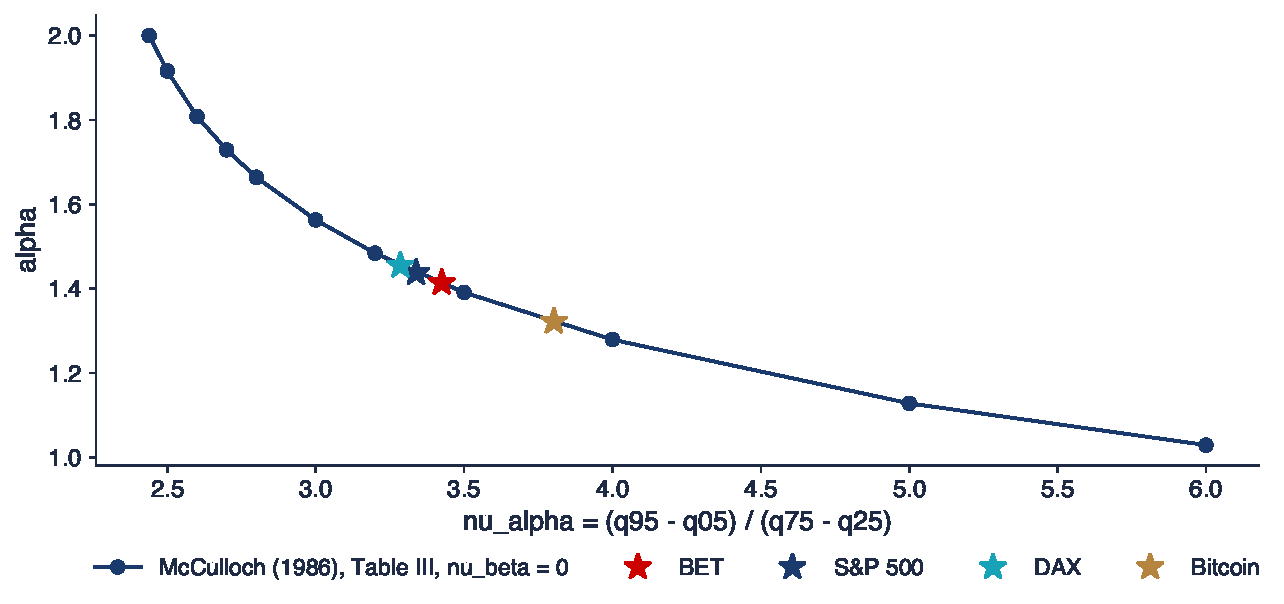
\includegraphics[width=\linewidth,height=0.78\textheight,keepaspectratio]{sfm_ch3_mcculloch_map.pdf}
\end{center}
\end{column}
\begin{column}{0.38\textwidth}
\begin{itemize}
    \item Linia: Tabelul III pentru un eșantion simetric ($\nu_\beta = 0$)
    \item Stelele: randamente logaritmice zilnice din 2000 (Bitcoin din 2014)
    \item $\nu_\alpha$: BET $3{,}425$, S\&P 500 $3{,}338$, DAX $3{,}285$, Bitcoin $3{,}803$
    \item Toate mult peste 2,439: cozi mult mai largi decît permite distribuția Normală
\end{itemize}
\end{column}
\end{columns}
\quantlet{SFM\_ch3\_estimation}{\qlurl{SFM_ch3_estimation}}
\end{frame}

\begin{frame}{Exemplu lucrat: McCulloch pe BET}
\itemsize{\small}
\begin{itemize}
    \item Randamentele logaritmice zilnice BET (\%), 2000--2026, $n = 6\,670$
    \item Pasul 1: cuantilele
    \begin{itemize}
        \item $\hat q_{0{,}05} = -1{,}93$, $\hat q_{0{,}25} = -0{,}50$, $\hat q_{0{,}5} = 0{,}08$, $\hat q_{0{,}75} = 0{,}66$, $\hat q_{0{,}95} = 2{,}06$
    \end{itemize}
    \item Pasul 2: rapoartele
    \begin{itemize}
        \item $\nu_\alpha = 4{,}00/1{,}17 = 3{,}425$; $\nu_\beta = -0{,}006$, practic simetric
    \end{itemize}
    \item Pasul 3: Tabelul III, coloana $\nu_\beta = 0$: $\nu_\alpha = 3{,}2 \mapsto 1{,}484$, $\nu_\alpha = 3{,}5 \mapsto 1{,}391$
    \begin{itemize}
        \item interpolare liniară: $\hat\alpha \approx 1{,}414$
    \end{itemize}
    \item Pasul 4: $\hat\gamma = 0{,}60$ (\% pe zi), $\hat\beta = -0{,}011$, $\hat\delta_0 = 0{,}079$
\end{itemize}\quantlet{SFM\_ch3\_estimation}{\qlurl{SFM_ch3_estimation}}
\end{frame}

\begin{frame}{Verosimilitatea maximă}
\itemsize{\small}
\begin{itemize}
    \item Log-verosimilitatea unui eșantion $r_1, \dots, r_n$: $\ell(\theta) = \sum_{t=1}^n \ln f(r_t; \theta)$, $\theta = (\alpha, \beta, \gamma, \delta_0)$
    \begin{itemize}
        \item $\theta$: vectorul celor patru parametri; $f(r_t; \theta)$: densitatea stabilă în $r_t$; $\hat\theta$ maximizează numeric $\ell$, pornind de la estimarea McCulloch
        \item erorile standard din curbura lui $\ell$: inversa hessianei, matricea derivatelor a doua ale lui $\ell$
    \end{itemize}
    \item Densitatea $f$ se calculează din $\varphi$
    \begin{itemize}
        \item $f(x) = \frac{1}{2\pi}\int e^{-itx}\varphi(t)\,dt$, evaluată pe o grilă cu FFT (fast Fourier transform, transformata Fourier rapidă) \refMDC
        \item sau prin integrare directă \refNolanA; \texttt{levy\_stable.fit} face acest calcul și durează cîteva minute pentru cîteva mii de randamente
    \end{itemize}
    \item Estimarea ML în S0 este regulată pentru $\alpha \in (0, 2)$: erorile standard scad ca $1/\sqrt{n}$ \refNolanML
\end{itemize}
\end{frame}

\begin{frame}{McCulloch și ML într-un studiu Monte Carlo}
\itemsize{\footnotesize}
\begin{center}
    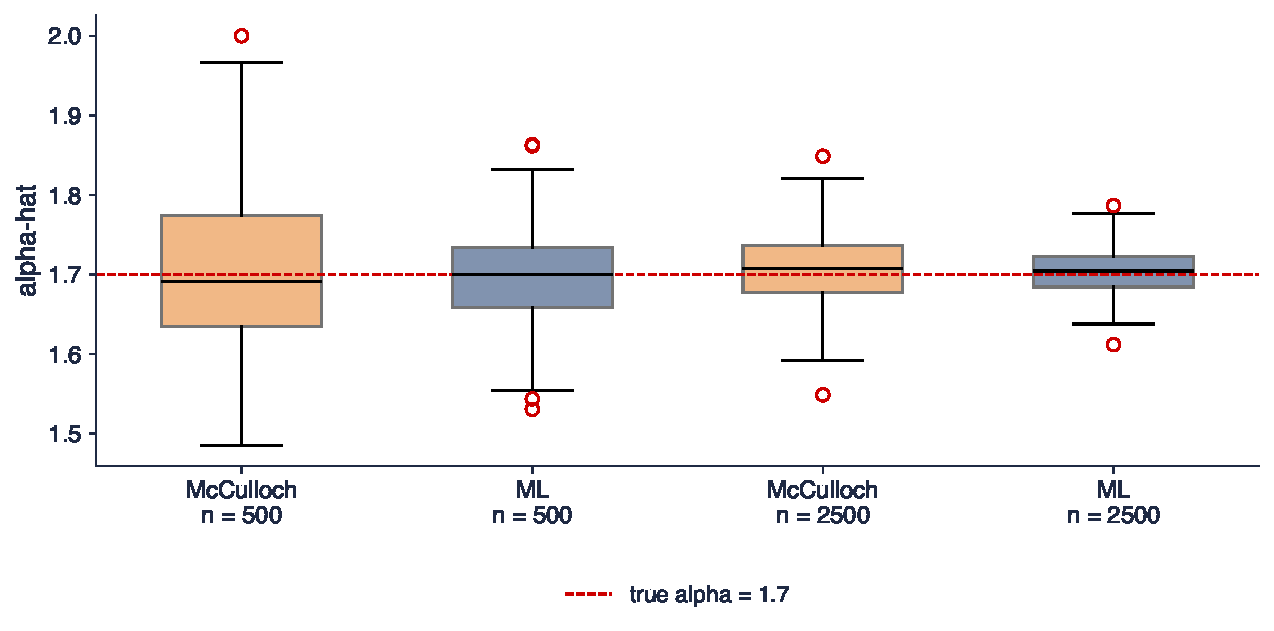
\includegraphics[width=0.97\textwidth,height=0.60\textheight,keepaspectratio]{sfm_ch3_estimators_mc.pdf}
\end{center}
\vspace{-0.25cm}
\begin{itemize}
    \item 200 de eșantioane din $S(1{,}7; 0; 1; 0)$ pentru fiecare mărime; ambii estimatori sînt centrați pe 1,7
    \item Abaterea standard a lui $\hat\alpha$: $n = 500$: McCulloch $0{,}107$, ML $0{,}061$; $n = 2500$: $0{,}046$ față de $0{,}030$
    \item ML este de circa $1{,}7$ ori mai precisă pe aceleași date
\end{itemize}
\quantlet{SFM\_ch3\_estimation}{\qlurl{SFM_ch3_estimation}}
\end{frame}

\begin{frame}{Recapitulare: estimarea}
\itemsize{\small}
\begin{itemize}
    \item McCulloch: cinci cuantile, două rapoarte, patru tabele; rapidă și robustă
    \item ML: densitate numerică din $\varphi$, maximizare numerică; cea mai precisă
    \item Raportați parametrizarea (S0 sau S1) și unitățile lui $\gamma$ și $\delta$
\end{itemize}
\end{frame}


%=============================================================================
\section{Estimarea pe randamente reale}
%=============================================================================

\begin{frame}{Legi stabile estimate pe randamentele logaritmice zilnice}
\itemsize{\small}
\begin{center}
\footnotesize
\begin{tabular}{lrrrrrrr}
\toprule
& $n$ & $\hat\alpha$ McC. & $\hat\alpha$ ML (SE) & $\hat\beta$ ML (SE) & $\hat\gamma$ & $\hat\delta_0$ & $\hat\delta_1$ \\
\midrule
BET & 6\,670 & $1{,}414$ & $1{,}486$ ($0{,}020$) & $-0{,}016$ ($0{,}034$) & $0{,}62$ & $0{,}088$ & $0{,}078$ \\
S\&P 500 & 6\,714 & $1{,}438$ & $1{,}540$ ($0{,}021$) & $-0{,}181$ ($0{,}036$) & $0{,}58$ & $0{,}093$ & $0{,}000$ \\
DAX & 6\,786 & $1{,}455$ & $1{,}606$ ($0{,}021$) & $-0{,}179$ ($0{,}040$) & $0{,}74$ & $0{,}090$ & $-0{,}004$ \\
Bitcoin & 4\,384 & $1{,}322$ & $1{,}410$ ($0{,}026$) & $0{,}019$ ($0{,}036$) & $1{,}54$ & $0{,}132$ & $0{,}171$ \\
\bottomrule
\end{tabular}
\end{center}
\begin{itemize}
    \item Randamente logaritmice zilnice în \%; indici 2000--2026, Bitcoin 2014--2026 (7 zile pe săptămînă); date: EODHD
    \item McC.: McCulloch; ML în S0, cu erori standard; $\hat\gamma$, $\hat\delta_0$, $\hat\delta_1$ în \% pe zi
\end{itemize}\quantlet{SFM\_ch3\_fit\_returns}{\qlurl{SFM_ch3_fit_returns}}
\end{frame}

\begin{frame}{Interpretarea estimărilor}
\itemsize{\small}
\begin{itemize}
    \item $\hat\alpha$ mult sub 2 pentru toate cele patru serii
    \begin{itemize}
        \item S\&P 500: $(2 - 1{,}540)/0{,}021 \approx 22$ erori standard față de cazul Normal
        \item cele mai groase cozi: Bitcoin ($\hat\alpha = 1{,}410$)
    \end{itemize}
    \item $\hat\beta < 0$ pentru S\&P 500 și DAX: coada stîngă este mai groasă (crahuri)
    \begin{itemize}
        \item BET și Bitcoin: $\hat\beta$ la mai puțin de două erori standard de 0
    \end{itemize}
    \item $\hat\gamma$: Bitcoin $1{,}54\%$ pe zi, față de $0{,}58\%$ pentru S\&P 500; comparați abaterile standard de selecție $3{,}49\%$ și $1{,}21\%$
    \item McCulloch dă un $\hat\alpha$ mai mic decît ML pentru fiecare serie: cele două metode ponderează diferit cozile
\end{itemize}
\end{frame}

\begin{frame}{Densități estimate, pe scară logaritmică}
\itemsize{\footnotesize}
\begin{center}
    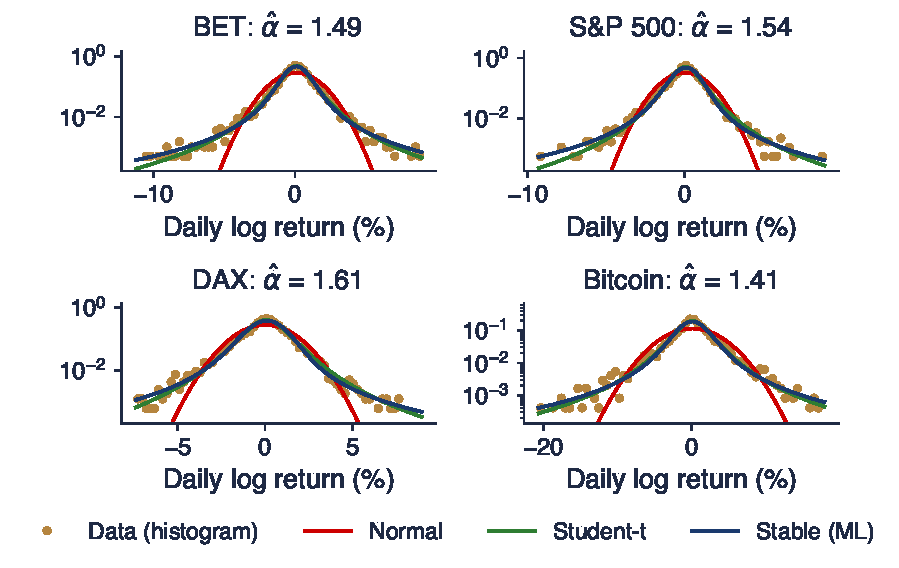
\includegraphics[width=0.97\textwidth,height=0.66\textheight,keepaspectratio]{sfm_ch3_fit_density.pdf}
\end{center}
\vspace{-0.25cm}
\begin{itemize}
    \item Distribuția Normală (roșu): mult prea puține randamente mari; distribuțiile Student-t (verde) și stabilă (albastru) descriu bine corpul
    \item Cozile îndepărtate: densitatea stabilă rămîne deasupra punctelor; distribuția Student-t este mai aproape de ele
\end{itemize}
\quantlet{SFM\_ch3\_fit\_returns}{\qlurl{SFM_ch3_fit_returns}}
\end{frame}

\begin{frame}{QQ plots față de cele trei modele}
\itemsize{\footnotesize}
\begin{center}
    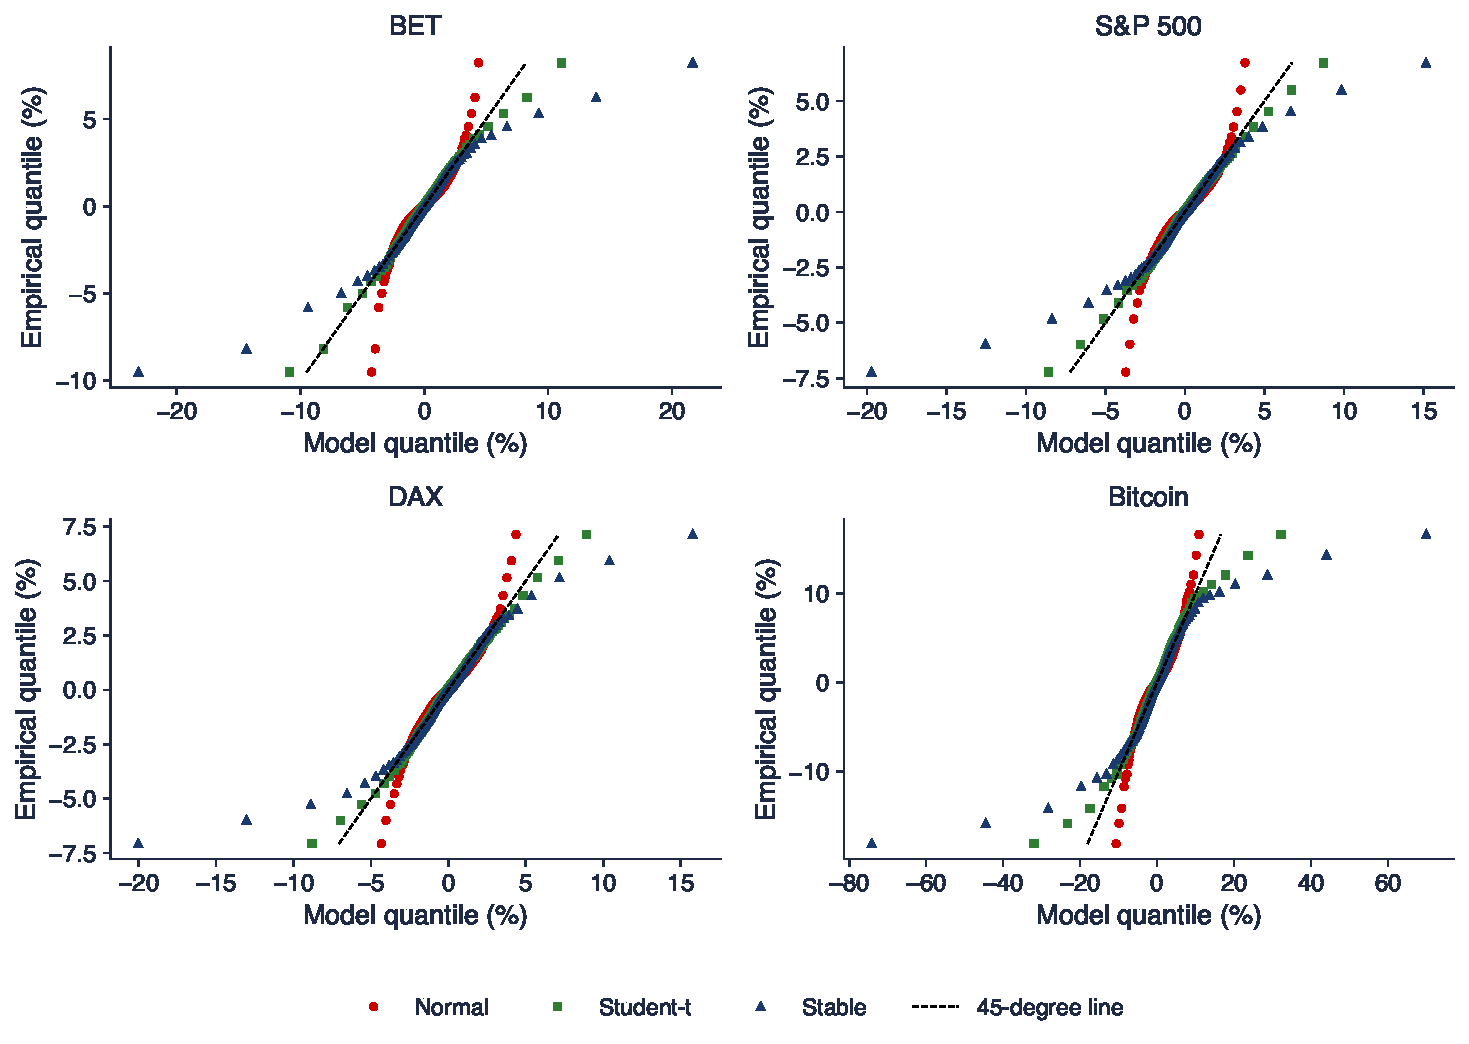
\includegraphics[width=0.97\textwidth,height=0.62\textheight,keepaspectratio]{sfm_ch3_qq_real.pdf}
\end{center}
\vspace{-0.25cm}
\begin{itemize}
    \item Un QQ plot (graficul cuantilă--cuantilă) reprezintă cuantilele empirice în funcție de cele ale modelului; pentru un model bun, punctele se află pe prima bisectoare
    \item Distribuția Normală: cozi prea scurte (capete abrupte); distribuția stabilă: cozi prea lungi (capete plate, cuantile ale modelului mult dincolo de date); Student-t: cea mai apropiată
\end{itemize}
\quantlet{SFM\_ch3\_fit\_returns}{\qlurl{SFM_ch3_fit_returns}}
\end{frame}

\begin{frame}{Coada stîngă pe axe log-log}
\itemsize{\footnotesize}
\begin{center}
    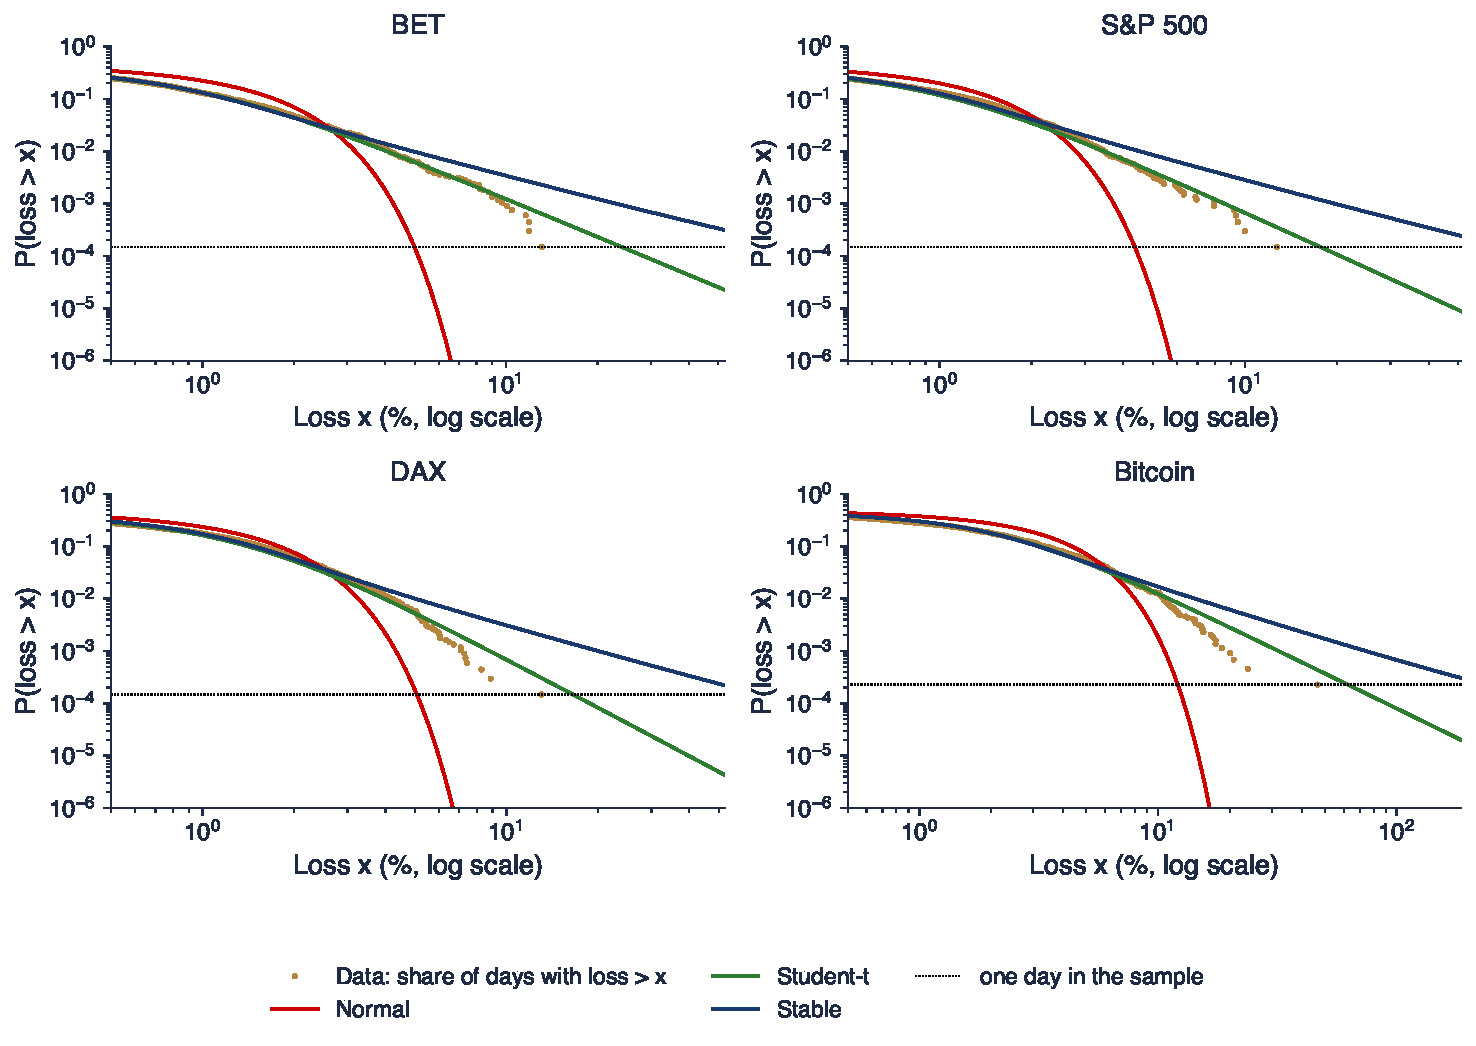
\includegraphics[width=0.97\textwidth,height=0.66\textheight,keepaspectratio]{sfm_ch3_tails_real.pdf}
\end{center}
\vspace{-0.25cm}
\begin{itemize}
    \item Punctele: proporția zilelor cu o pierdere peste $x$; liniile: aceeași probabilitate conform fiecărui model estimat
    \item Coada empirică se curbează în jos mai repede decît dreapta stabilă: tail index-ul datelor este mai mare decît $\hat\alpha$
\end{itemize}
\quantlet{SFM\_ch3\_fit\_returns}{\qlurl{SFM_ch3_fit_returns}}
\end{frame}

\begin{frame}{Numărarea pierderilor mari}
\itemsize{\small}
\begin{center}
\footnotesize
\begin{tabular}{lrrrrr}
\toprule
& pierdere peste & observate & Normală & Student-t & stabilă \\
\midrule
S\&P 500 & $5\%$ & 23 & $0{,}1$ & $27{,}0$ & $57{,}3$ \\
S\&P 500 & $10\%$ & 1 & $\approx 0$ & $4{,}5$ & $19{,}1$ \\
S\&P 500 & $15\%$ & 0 & $\approx 0$ & $1{,}5$ & $10{,}2$ \\
BET & $10\%$ & 6 & $\approx 0$ & $8{,}2$ & $22{,}8$ \\
Bitcoin & $10\%$ & 56 & $8{,}1$ & $54{,}2$ & $73{,}9$ \\
Bitcoin & $20\%$ & 4 & $\approx 0$ & $12{,}3$ & $26{,}9$ \\
\bottomrule
\end{tabular}
\end{center}
\begin{itemize}
    \item Numărul așteptat de zile $= n \times P(r < -x)$ conform fiecărui model estimat
    \item Distribuția Normală: aproape nicio pierdere mare; distribuția stabilă: prea multe, iar diferența crește odată cu pragul; Student-t: cea mai apropiată de valorile observate
    \item S\&P 500, 6\,714 zile: zile sub $-10\%$ observate 1, prevăzute de legea stabilă estimată $19{,}1$
\end{itemize}\quantlet{SFM\_ch3\_fit\_returns}{\qlurl{SFM_ch3_fit_returns}}
\end{frame}

\begin{frame}{VaR 1\% și VaR 0,1\% conform celor trei modele}
\itemsize{\small}
\begin{center}
\footnotesize
\begin{tabular}{l|rrrr|rrrr}
\toprule
& \multicolumn{4}{c|}{VaR 1\% (\%)} & \multicolumn{4}{c}{VaR 0,1\% (\%)} \\ & date & Normală & t & stabilă & date & Normală & t & stabilă \\
\midrule
BET & $4{,}1$ & $3{,}2$ & $4{,}1$ & $4{,}9$ & $9{,}5$ & $4{,}3$ & $10{,}9$ & $23{,}1$ \\
S\&P 500 & $3{,}5$ & $2{,}8$ & $3{,}5$ & $4{,}5$ & $7{,}2$ & $3{,}7$ & $8{,}6$ & $19{,}7$ \\
DAX & $4{,}2$ & $3{,}3$ & $4{,}0$ & $5{,}0$ & $7{,}1$ & $4{,}3$ & $8{,}8$ & $20{,}0$ \\
Bitcoin & $10{,}5$ & $8{,}0$ & $11{,}1$ & $14{,}3$ & $18{,}1$ & $10{,}7$ & $31{,}9$ & $74{,}2$ \\
\bottomrule
\end{tabular}
\end{center}
\begin{itemize}
    \item VaR la nivelul $p$: $\mathrm{VaR}_p = -q_p$, pierderea zilnică depășită cu probabilitatea $p$ (\sfmchlink{https://danpele.github.io/SFM/RO/Cursuri/capitol10_var_es_backtesting.pdf}{Capitolul 10}); aici notăm nivelul cu $p$, deoarece $\alpha$ desemnează indicele de stabilitate
    \item VaR 1\%: modelul Normal dă valori prea mici, modelul stabil valori prea mari
    \item VaR 0,1\%: modelul stabil dă valori de aproximativ două pînă la patru ori mai mari decît cuantila empirică
\end{itemize}\quantlet{SFM\_ch3\_fit\_returns}{\qlurl{SFM_ch3_fit_returns}}
\end{frame}

\begin{frame}{Compararea celor trei modele}
\itemsize{\small}
\begin{center}
\footnotesize
\begin{tabular}{lrrrr}
\toprule
& AIC Normală & AIC Student-t & AIC stabilă & $\hat\nu$ (Student-t) \\
\midrule
BET & 23\,407 & 20\,996 & 21\,088 & $2{,}43$ \\
S\&P 500 & 21\,650 & 19\,702 & 19\,794 & $2{,}67$ \\
DAX & 23\,901 & 22\,595 & 22\,697 & $3{,}09$ \\
Bitcoin & 23\,391 & 22\,056 & 22\,159 & $2{,}23$ \\
\bottomrule
\end{tabular}
\end{center}
\begin{itemize}
    \item AIC (Akaike information criterion, criteriul informațional Akaike) $= 2k - 2\ell(\hat\theta)$, cu $k$ numărul de parametri; se preferă valoarea mai mică
    \item Ambele modele cu cozi groase sînt preferate distribuției Normale, cu diferențe de mii de puncte AIC
    \item Student-t este preferată pentru fiecare serie, deși are mai puțini parametri; la S\&P 500, diferența este de 92 de puncte
    \item $\hat\nu$ între 2 și 3,1: varianță finită, dar aproape niciun moment finit de ordin superior
\end{itemize}\quantlet{SFM\_ch3\_fit\_returns}{\qlurl{SFM_ch3_fit_returns}}
\end{frame}

\begin{frame}{Recapitulare: estimarea pe randamente reale}
\itemsize{\small}
\begin{itemize}
    \item Toate cele patru serii: $\hat\alpha$ între 1{,}410 și 1{,}606, departe de 2
    \item Legea stabilă descrie corpul distribuției mult mai bine decît distribuția Normală
    \item Supraestimează cozile îndepărtate: prea multe pierderi extreme, VaR 0,1\% prea mare
    \item După AIC, distribuția Student-t este preferată
\end{itemize}
\end{frame}


%=============================================================================
\section{Critica: varianță finită sau infinită?}
%=============================================================================

\begin{frame}{Testul 1: rămîne $\alpha$ la fel cînd randamentele se adună?}
\itemsize{\footnotesize}
\begin{center}
    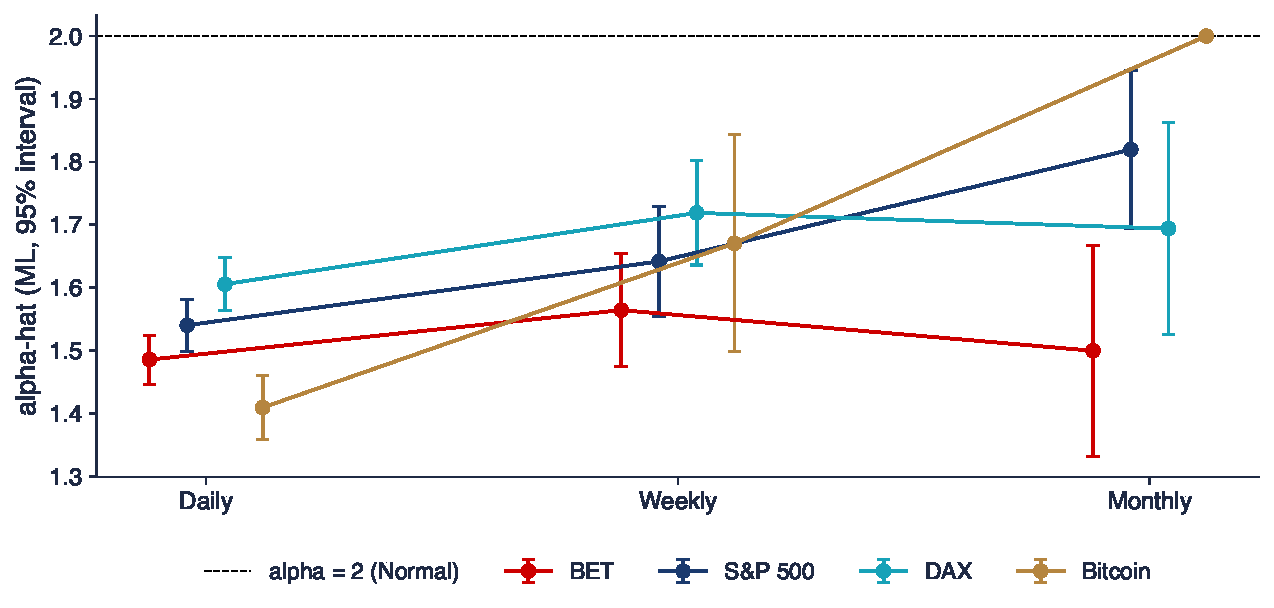
\includegraphics[width=0.97\textwidth,height=0.64\textheight,keepaspectratio]{sfm_ch3_aggregation.pdf}
\end{center}
\vspace{-0.25cm}
\begin{itemize}
    \item Dacă randamentele zilnice ar fi i.i.d.\ stabile, sumele săptămînale și lunare ar avea \textbf{același} $\alpha$ (stabilitatea)
    \item Estimări ML: S\&P 500 $1{,}54 \to 1{,}64 \to 1{,}82$; Bitcoin $1{,}41 \to 1{,}67 \to 2{,}00$ (la limita 2)
\end{itemize}
\quantlet{SFM\_ch3\_aggregation}{\qlurl{SFM_ch3_aggregation}}
\end{frame}

\begin{frame}{Interpretarea testului de agregare}
\itemsize{\small}
\begin{itemize}
    \item $\hat\alpha$ crește cu orizontul pentru S\&P 500, DAX și Bitcoin
    \begin{itemize}
        \item DAX: $1{,}61 \to 1{,}72 \to 1{,}69$; pentru S\&P 500, intervalele de încredere ale orizontului zilnic și lunar nu se suprapun
    \end{itemize}
    \item BET: $1{,}49 \to 1{,}56 \to 1{,}50$, fără o creștere clară
    \begin{itemize}
        \item eșantioanele lunare sînt scurte (321 de luni): intervale largi
    \end{itemize}
    \item Același tipar în studiile clasice: \refOfficer, \refAB
    \item Un $\alpha$ crescător este exact ceea ce prevede GCLT pentru sume de randamente cu varianță finită care converg lent la distribuția Normală
\end{itemize}
\end{frame}

\begin{frame}{Testul 2: se stabilizează varianța de selecție?}
\itemsize{\footnotesize}
\begin{center}
    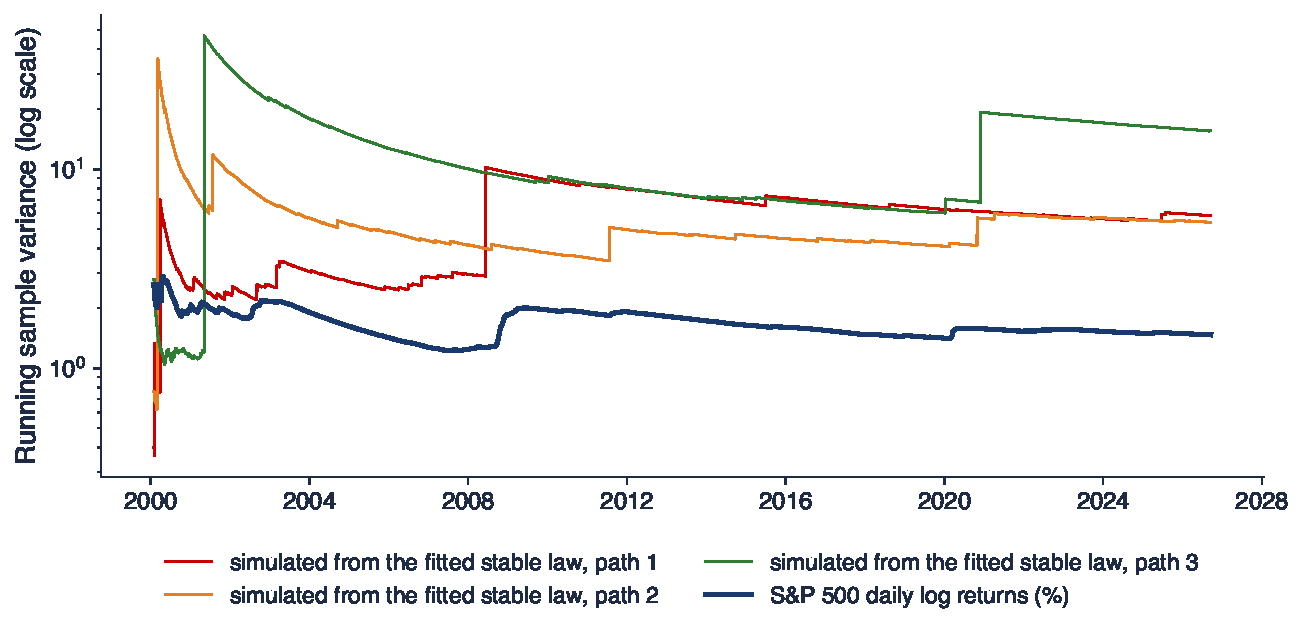
\includegraphics[width=0.97\textwidth,height=0.64\textheight,keepaspectratio]{sfm_ch3_running_var_real.pdf}
\end{center}
\vspace{-0.25cm}
\begin{itemize}
    \item S\&P 500 (albastru): după salturile din 2008 și 2020, varianța cumulată se stabilizează în jur de $1{,}47$
    \item Traiectorii de aceeași lungime simulate din legea stabilă estimată: varianțe finale între $5{,}4$ și $15{,}6$, mult peste date
\end{itemize}
\quantlet{SFM\_ch3\_aggregation}{\qlurl{SFM_ch3_aggregation}}
\end{frame}

\begin{frame}{Testul 3: cît de groasă este coada îndepărtată?}
\itemsize{\small}
\begin{itemize}
    \item $\alpha$ stabil este determinat de întreaga distribuție, mai ales de corp
    \begin{itemize}
        \item tail index-ul cozii îndepărtate se estimează separat, cu estimatorul Hill \refHill\ (\sfmchlink{https://danpele.github.io/SFM/RO/Cursuri/capitol5_cozi_groase_evt.pdf}{Capitolul 5})
    \end{itemize}
    \item Pentru indicii bursieri, coada îndepărtată scade aproximativ ca $x^{-3}$, „legea cubică inversă” \refGopi
    \begin{itemize}
        \item un tail index în jur de 3 înseamnă varianță finită, iar nicio lege stabilă nu îl are
    \end{itemize}
    \item Numărul pierderilor observate confirmă: legile stabile estimate prevăd mult mai multe pierderi peste $10\%$ decît s-au observat
    \item \refLLW: alte dovezi împotriva modelului stabil, din comportamentul momentelor de selecție
\end{itemize}
\end{frame}

\begin{frame}{Originea aspectului stabil al randamentelor zilnice}
\itemsize{\small}
\begin{itemize}
    \item \textbf{Volatility clustering} (\sfmchlink{https://danpele.github.io/SFM/RO/Cursuri/capitol2_distributii_clasice_fapte_stilizate.pdf}{Capitolele 2} și \sfmchlink{https://danpele.github.io/SFM/RO/Cursuri/capitol9_modele_arch_garch.pdf}{9}): perioadele calme și cele agitate alternează
    \begin{itemize}
        \item un amestec de legi Normale cu varianță variabilă are cozi groase și varianță finită \refBG
        \item dacă pe datele generate de amestec se estimează o singură lege stabilă, se obține $\hat\alpha < 2$
    \end{itemize}
    \item \textbf{Legi stabile trunchiate și temperate}: stabile la scări moderate, cu cozi mai subțiri în zona extremă
    \begin{itemize}
        \item \refMS\ au estimat un zbor Lévy trunchiat (truncated Lévy flight) pe S\&P 500
        \item \refGS: astfel de legi explică de ce randamentele par stabile pe orizonturi scurte și Normale pe orizonturi lungi
    \end{itemize}
\end{itemize}
\end{frame}

\begin{frame}{Verdictul}
\itemsize{\small}
\begin{itemize}
    \item \textbf{Mandelbrot a avut dreptate} în privința faptelor
    \begin{itemize}
        \item randamentele zilnice au cozi groase; distribuția Normală descrie foarte slab datele
    \end{itemize}
    \item \textbf{Varianța infinită nu este susținută}
    \begin{itemize}
        \item $\hat\alpha$ crește prin agregare; varianța de selecție se stabilizează; coada îndepărtată este mai subțire decît orice coadă stabilă
    \end{itemize}
    \item Unde rămîn utile legile stabile
    \begin{itemize}
        \item un etalon pentru cozi groase; simulare; ideea de scalare; date cu varianță cu adevărat infinită (unele daune de asigurări, unele tokenuri cripto)
        \item GCLT: o reamintire că regulile cu $\sqrt{n}$ cer varianță finită
    \end{itemize}
    \item Urmează: \sfmchlink{https://danpele.github.io/SFM/RO/Cursuri/capitol5_cozi_groase_evt.pdf}{Capitolul 5} estimează direct tail index-ul cu teoria valorilor extreme
\end{itemize}
\end{frame}

\begin{frame}{Recapitulare: critica}
\itemsize{\small}
\begin{itemize}
    \item Stabilitatea implică același $\alpha$ la orice orizont: datele arată un $\alpha$ crescător
    \item Varianța de selecție a randamentelor reale se stabilizează; cea a eșantioanelor stabile, nu
    \item Volatility clustering și cozile temperate explică valoarea aparentă $\alpha < 2$
    \item Cozi groase: da; varianță infinită: nu
\end{itemize}
\end{frame}


%=============================================================================
\section{AI pentru descoperire științifică}
%=============================================================================

\begin{frame}{O întrebare deschisă}
\itemsize{\small}
\begin{itemize}
    \item \textbf{Au devenit mai subțiri cozile Bitcoin pe măsură ce piața s-a maturizat?}
    \begin{itemize}
        \item mai mulți participanți, contracte futures și ETF-uri (exchange-traded funds, fonduri tranzacționate la bursă) în perioada 2017--2024
        \item dacă cozile au devenit mai subțiri, modelele de risc estimate pe date vechi supraestimează riscul de azi
    \end{itemize}
    \item De ce rămîne deschisă: $\hat\alpha$ variază odată cu regimurile de volatilitate, iar eșantioanele anuale sînt scurte
    \item Eșantionul complet: $\hat\alpha = 1{,}410$ (SE $0{,}026$), cel mai mic dintre cele patru serii
    \item Instrumentele AI pot accelera un astfel de studiu; nu înlocuiesc verificarea lui \refWang
\end{itemize}
\end{frame}

\begin{frame}{Contribuția posibilă a AI}
\itemsize{\small}
\begin{itemize}
    \item \textbf{Literatura}: inventarierea lucrărilor despre estimarea cozilor activelor cripto și rezumarea metodelor lor
    \item \textbf{Cod}: o primă versiune a unui estimator McCulloch pe ferestre mobile, cu intervale bootstrap
    \item \textbf{Robustețe}: propunerea altor ferestre, ML în loc de cuantile, $\nu$ din Student-t în loc de $\alpha$
    \item \textbf{Explicație}: o primă versiune a interpretării unui tabel de estimări anuale
    \item Exemplu de prompt
    \begin{itemize}
        \item \aiprompt{Write a Python function that estimates the stable alpha of daily log returns on rolling 365-day windows with McCulloch (1986), and adds 95\% bootstrap intervals.}
    \end{itemize}
\end{itemize}
\end{frame}

\begin{frame}{Verificări necesare}
\itemsize{\small}
\begin{itemize}
    \item Parametrizarea: S0 sau S1; scipy folosește implicit S1; poziția diferă cu $\beta\gamma\tan\frac{\pi\alpha}{2}$
    \item Unitățile: randamente în \% sau în zecimale; $\gamma$ și $\delta$ se schimbă, $\alpha$ și $\beta$ nu
    \item Ferestrele suprapuse nu sînt independente: nu citiți estimările mobile ca teste separate
    \item Rezultatele numerice: recalculați o fereastră cu o a doua metodă (ML sau tabelele de cuantile)
    \item Referințele: fiecare lucrare citată trebuie să existe; verificați DOI-ul
\end{itemize}
\end{frame}

\begin{frame}{Idee de proiect}
\itemsize{\small}
\begin{itemize}
    \item \textbf{Întrebarea}: este coada randamentelor Bitcoin mai subțire acum decît în 2014--2018?
    \begin{itemize}
        \item date: prețurile de închidere zilnice ale Bitcoin din datele cursului (EODHD), 2014--2026
    \end{itemize}
    \item Pași
    \begin{itemize}
        \item estimați $\alpha$ prin McCulloch și prin ML pentru fiecare an calendaristic, cu intervale bootstrap
        \item repetați pe randamente împărțite la o volatilitate mobilă: se menține tendința?
        \item comparați cu $\hat\nu$ din Student-t pentru fiecare an
    \end{itemize}
    \item Livrabile: un tabel, un grafic și un paragraf despre ce pot și ce nu pot arăta datele
    \item Declarați orice folosire a AI și listați erorile AI pe care le-ați corectat
\end{itemize}
\end{frame}


%=============================================================================
\section{Rezumat}
%=============================================================================

\begin{frame}{Idei principale}
\itemsize{\small}
\begin{itemize}
    \item Legile stabile sînt singurele legi ale căror sume își păstrează forma și singurele limite ale sumelor normalizate (GCLT)
    \item Patru parametri: $\alpha$ cozi, $\beta$ asimetrie, $\gamma$ scală, $\delta$ poziție; precizați întotdeauna parametrizarea (S0 sau S1)
    \item $\alpha < 2$: cozi de tip putere și varianță infinită; $\alpha \le 1$: nu există media
    \item Simulați cu CMS; estimați cu cuantilele McCulloch sau cu ML
    \item Randamentele zilnice: $\hat\alpha \approx 1{,}4$--$1{,}6$; legea stabilă descrie corpul distribuției mult mai bine decît distribuția Normală
    \item Dar $\hat\alpha$ crește prin agregare, iar varianța se stabilizează: cozi groase, varianță finită
\end{itemize}
\end{frame}

\begin{frame}{Formule de reținut}
\itemsize{\small}
{\renewcommand{\arraystretch}{1.45}\begin{center}
\scriptsize
\begin{tabular}{ll}
\toprule
\textbf{Mărimea} & \textbf{Formula} \\
\midrule
Stabilitate & $aX_1 + bX_2 \overset{d}{=} cX + d$, \quad $c^\alpha = a^\alpha + b^\alpha$ \\
Suma a $n$ copii & $X_1 + \dots + X_n \overset{d}{=} n^{1/\alpha}X + d_n$ \\
Funcția caracteristică (S1) & $\exp\{-\gamma^\alpha|t|^\alpha[1 - i\beta\,\mathrm{sign}(t)\tan\frac{\pi\alpha}{2}] + i\delta_1 t\}$ \\
S0 și S1 & $\delta_0 = \delta_1 + \beta\gamma\tan\frac{\pi\alpha}{2}$ \\
Cazul Normal & $S(2; \beta; \gamma; \delta) = N(\delta, 2\gamma^2)$ \\
Cozi & $P(X > x) \sim \gamma^\alpha c_\alpha(1 + \beta)x^{-\alpha}$ \\
Momente & $E|X|^p < \infty \iff p < \alpha$ \quad ($\alpha < 2$) \\
CMS ($\beta = 0$) & $\dfrac{\sin(\alpha V)}{(\cos V)^{1/\alpha}}\Big(\dfrac{\cos((1-\alpha)V)}{W}\Big)^{(1-\alpha)/\alpha}$ \\
McCulloch & $\nu_\alpha = \dfrac{q_{0{,}95} - q_{0{,}05}}{q_{0{,}75} - q_{0{,}25}}$, \quad $\nu_\beta = \dfrac{q_{0{,}95} + q_{0{,}05} - 2q_{0{,}5}}{q_{0{,}95} - q_{0{,}05}}$ \\
\bottomrule
\end{tabular}
\end{center}
}
\end{frame}

\begin{frame}{Autoevaluare}
\itemsize{\small}
\begin{itemize}
    \item \textbf{Întrebare}: randamentele zilnice sînt i.i.d.\ $S(1{,}5; 0; \gamma; 0)$; de cîte ori crește scala de la 1 zi la 20 de zile?
    \begin{itemize}
        \item \textbf{Răspuns}: $20^{1/1{,}5} = 7{,}37$, adică de $1{,}65$ ori mai mult decît factorul $\sqrt{20}$ al regulii rădăcinii pătrate a timpului
    \end{itemize}
    \item \textbf{Întrebare}: o lege estimată are $\alpha = 1{,}2$; există media și varianța?
    \begin{itemize}
        \item \textbf{Răspuns}: media există ($1 < 1{,}2$), varianța nu ($2 > 1{,}2$)
    \end{itemize}
    \item \textbf{Întrebare}: scipy raportează $\delta = 0{,}05$ cu $\alpha = 1{,}7$, $\beta = -0{,}2$, $\gamma = 0{,}6$; cît este $\delta_0$?
    \begin{itemize}
        \item \textbf{Răspuns}: scipy folosește S1, deci $\delta_0 = 0{,}05 + (-0{,}2)(0{,}6)\tan(0{,}85\pi) = 0{,}05 + 0{,}061 = 0{,}111$
    \end{itemize}
    \item Urmează: \sfmchlink{https://danpele.github.io/SFM/RO/Cursuri/capitol4_probabilitate.pdf}{Capitolul 4}, probabilități pentru finanțe
\end{itemize}
\end{frame}


%=============================================================================
\section{Bibliografie}
%=============================================================================

\begin{frame}{Bibliografie (1/2)}
\itemsize{\tiny}
\begin{itemize}
    \item Akgiray, V., Booth, G.G. (1988). \href{https://doi.org/10.1080/07350015.1988.10509636}{The stable-law model of stock returns}. \textit{Journal of Business \& Economic Statistics}, 6(1), 51--57.
    \item Blattberg, R.C., Gonedes, N.J. (1974). \href{https://doi.org/10.1086/295634}{A comparison of the stable and Student distributions as statistical models for stock prices}. \textit{Journal of Business}, 47(2), 244--280.
    \item Borak, S., Härdle, W., Weron, R. (2005). \href{https://doi.org/10.1007/3-540-27395-6_1}{Stable distributions}. In Čížek, P., Härdle, W., Weron, R. (eds.), \textit{Statistical Tools for Finance and Insurance}, 21--44. Springer.
    \item Borak, S., Misiorek, A., Weron, R. (2011). \href{https://doi.org/10.1007/978-3-642-18062-0_1}{Models for heavy-tailed asset returns}. In Čížek, P., Härdle, W.K., Weron, R. (eds.), \textit{Statistical Tools for Finance and Insurance}, 2nd ed., 21--55. Springer.
    \item Chambers, J.M., Mallows, C.L., Stuck, B.W. (1976). \href{https://doi.org/10.1080/01621459.1976.10480344}{A method for simulating stable random variables}. \textit{Journal of the American Statistical Association}, 71(354), 340--344.
    \item Cont, R. (2001). \href{https://doi.org/10.1080/713665670}{Empirical properties of asset returns: stylized facts and statistical issues}. \textit{Quantitative Finance}, 1(2), 223--236.
    \item Fama, E.F. (1965). \href{https://doi.org/10.1086/294743}{The behavior of stock-market prices}. \textit{Journal of Business}, 38(1), 34--105.
    \item Fama, E.F., Roll, R. (1968). \href{https://doi.org/10.1080/01621459.1968.11009311}{Some properties of symmetric stable distributions}. \textit{Journal of the American Statistical Association}, 63(323), 817--836.
    \item Fama, E.F., Roll, R. (1971). \href{https://doi.org/10.1080/01621459.1971.10482264}{Parameter estimates for symmetric stable distributions}. \textit{Journal of the American Statistical Association}, 66(334), 331--338.
    \item Franke, J., Härdle, W.K., Hafner, C.M. (2019). \href{https://doi.org/10.1007/978-3-030-13751-9}{\textit{Statistics of Financial Markets: An Introduction}}, 5th ed. Springer.
    \item Gnedenko, B.V., Kolmogorov, A.N. (1954). \href{https://archive.org/details/limitdistributio00gned_0}{\textit{Limit Distributions for Sums of Independent Random Variables}}. Addison-Wesley.
    \item Gopikrishnan, P., Plerou, V., Amaral, L.A.N., Meyer, M., Stanley, H.E. (1999). \href{https://doi.org/10.1103/PhysRevE.60.5305}{Scaling of the distribution of fluctuations of financial market indices}. \textit{Physical Review E}, 60(5), 5305--5316.
    \item Grabchak, M., Samorodnitsky, G. (2010). \href{https://doi.org/10.1080/14697680903540381}{Do financial returns have finite or infinite variance? A paradox and an explanation}. \textit{Quantitative Finance}, 10(8), 883--893.
    \item Hill, B.M. (1975). \href{https://doi.org/10.1214/aos/1176343247}{A simple general approach to inference about the tail of a distribution}. \textit{Annals of Statistics}, 3(5), 1163--1174.
    \item Koutrouvelis, I.A. (1980). \href{https://doi.org/10.1080/01621459.1980.10477573}{Regression-type estimation of the parameters of stable laws}. \textit{Journal of the American Statistical Association}, 75(372), 918--928.
    \item Lau, A.H.-L., Lau, H.-S., Wingender, J.R. (1990). \href{https://doi.org/10.1080/07350015.1990.10509793}{The distribution of stock returns: new evidence against the stable model}. \textit{Journal of Business \& Economic Statistics}, 8(2), 217--223.
\end{itemize}
\end{frame}

\begin{frame}{Bibliografie (2/2)}
\itemsize{\tiny}
\begin{itemize}
    \item Mandelbrot, B. (1963). \href{https://doi.org/10.1086/294632}{The variation of certain speculative prices}. \textit{Journal of Business}, 36(4), 394--419.
    \item Mantegna, R.N., Stanley, H.E. (1995). \href{https://doi.org/10.1038/376046a0}{Scaling behaviour in the dynamics of an economic index}. \textit{Nature}, 376(6535), 46--49.
    \item McCulloch, J.H. (1986). \href{https://doi.org/10.1080/03610918608812563}{Simple consistent estimators of stable distribution parameters}. \textit{Communications in Statistics -- Simulation and Computation}, 15(4), 1109--1136.
    \item Mittnik, S., Doganoglu, T., Chenyao, D. (1999). \href{https://doi.org/10.1016/S0895-7177(99)00106-5}{Computing the probability density function of the stable Paretian distribution}. \textit{Mathematical and Computer Modelling}, 29(10--12), 235--240.
    \item Mittnik, S., Rachev, S.T., Doganoglu, T., Chenyao, D. (1999). \href{https://doi.org/10.1016/S0895-7177(99)00110-7}{Maximum likelihood estimation of stable Paretian models}. \textit{Mathematical and Computer Modelling}, 29(10--12), 275--293.
    \item Nolan, J.P. (1997). \href{https://doi.org/10.1080/15326349708807450}{Numerical calculation of stable densities and distribution functions}. \textit{Communications in Statistics. Stochastic Models}, 13(4), 759--774.
    \item Nolan, J.P. (2001). \href{https://doi.org/10.1007/978-1-4612-0197-7_17}{Maximum likelihood estimation and diagnostics for stable distributions}. In Barndorff-Nielsen, O.E., Mikosch, T., Resnick, S.I. (eds.), \textit{Lévy Processes}, 379--400. Birkhäuser.
    \item Nolan, J.P. (2020). \href{https://doi.org/10.1007/978-3-030-52915-4}{\textit{Univariate Stable Distributions: Models for Heavy Tailed Data}}. Springer.
    \item Officer, R.R. (1972). \href{https://doi.org/10.1080/01621459.1972.10481297}{The distribution of stock returns}. \textit{Journal of the American Statistical Association}, 67(340), 807--812.
    \item Pele, D.T. (2014). \href{https://doi.org/10.1016/S2212-5671(14)00279-2}{A SAS approach for estimating the parameters of an alpha-stable distribution}. \textit{Procedia Economics and Finance}, 10, 68--77.
    \item Rachev, S.T., Mittnik, S. (2000). \href{https://www.wiley.com/en-us/Stable+Paretian+Models+in+Finance-p-9780471953142}{\textit{Stable Paretian Models in Finance}}. Wiley.
    \item Samorodnitsky, G., Taqqu, M.S. (1994). \href{https://doi.org/10.1201/9780203738818}{\textit{Stable Non-Gaussian Random Processes: Stochastic Models with Infinite Variance}}. Chapman \& Hall.
    \item Wang, H., Fu, T., Du, Y., Gao, W., et al. (2023). \href{https://doi.org/10.1038/s41586-023-06221-2}{Scientific discovery in the age of artificial intelligence}. \textit{Nature}, 620, 47--60.
    \item Weron, R. (1996). \href{https://doi.org/10.1016/0167-7152(95)00113-1}{On the Chambers--Mallows--Stuck method for simulating skewed stable random variables}. \textit{Statistics \& Probability Letters}, 28(2), 165--171.
\end{itemize}
\end{frame}

\end{document}
